% !TEX TS-program = lualatex+se
% !TEX encoding = UTF-8

\documentclass[oneside, 12pt, a4paper]{book}
%\usepackage[letterpaper,showframe]{geometry}
\usepackage{fullpage} % redukcja marginesów
\usepackage{geometry}
\geometry{
	left=15mm,
	right=10mm,
	top=12mm,
	bottom=15mm,
	marginparwidth=0mm,
	marginparsep=0mm
	}
\usepackage{gregoriotex}
\gresetlinecolor{gregoriocolor}
\gresetheadercapture{annotation}{greannotation}{string}
% Format annotation above initial
\grechangestyle{annotation}{\small\bfseries}%
\grechangedim{intersyllablespacenotes}{0.18cm}{scalable}%

\usepackage[hyperindex=true]{hyperref}
\usepackage{imakeidx}
\makeindex[title=Alfabetyczny spis program=texindy,options=-M styl.xdy]

\usepackage{filecontents}
\begin{filecontents*}{styl.xdy}
;;; xindy style file
(markup-locclass-list :open "\dotfill" :sep "")
(define-attributes (( "textbf" "default" )) )
(markup-locref   :attr  "textbf"     :open "\textbf{\hyperpage{" :close "}}")
(markup-locref   :attr  "textit"     :open "\textit{\hyperpage{" :close "}}")
(markup-locref   :attr  "textttt"     :open "\textttt{\hyperpage{" :close "}}")
(markup-locref   :attr  "texttsc"     :open "\texttsc{\hyperpage{" :close "}}")
(markup-locref   :attr  "default"     :open "\hyperpage{" :close "}")
\end{filecontents*}

\usepackage{fullpage}
\usepackage{multicol}

%  Konfiguracja kolumn
\usepackage{paracol}
\setcolumnwidth{14cm,4cm}
\setlength{\columnsep}{0.5cm}
\footnotelayout{m}
% \setlength{\columnseprule}{0.4pt}
% \colseprulecolor{red}
\usepackage{tcolorbox}
\newtcolorbox{nutybox}{size=minimal, colback=white, colframe=red, arc=0mm, width=\linewidth, halign=left, valign=center}
\newtcolorbox{tlumbox}{size=minimal, colback=white, colframe=red, arc=0mm, width=\linewidth, halign=left, valign=top}

\usepackage{Tabbing}
\usepackage{longtable}
\usepackage[savepos]{zref}

\let\grelocalleftbox\localleftbox
\let\grelocalrightbox\localrightbox

\usepackage[latin,polish]{babel}

\usepackage{fontspec}
\defaultfontfeatures{Ligatures=TeX}
\setmainfont{Libertinus Serif}

\pagestyle{plain}	% usuwanie nagłówków/stopek z\,dokumentu
\usepackage[indent=0pt]{parskip} % ustawianie paragrafów
%\usepackage{setspace} % odstępy między liniami
%\setstretch{1.5} % półtorej linii odległości między wierszami

\usepackage{graphicx} % umożliwia import obrazów
\graphicspath{{img/}} % katalog obrazów
\usepackage{pgfornament}% ornamenty graficzne

\usepackage{titlesec} % ustawianie nagłówków

\newfontface\vectis{VectisMonumentalW01-Regular}
\def\greinitialformat#1{\fontsize{20}{20}\vectis #1}

% --- komendy własne ---
\newcommand{\red}[1]{\textcolor{red}{#1}}
\newcommand{\black}[1]{\textcolor{black}{#1}}

\newcommand{\koniec}{
	\begin{center}
%		\vspace{5mm}
%		\pgfornament[width=0.6cm]{#1}
		\newpage
	\end{center}}

\begin{document}
\titlespacing*{\chapter}{0pt}{0pt}{5pt}	
\titleformat{\chapter}[hang]{\filcenter\LARGE\scshape\bfseries}{}{0pt}{} % format nagłówków
\titlespacing*{\section}{0pt}{0pt}{0pt}	
\titleformat{\section}[hang]{\filcenter\large\scshape}{}{0pt}{} % format nagłówków

\setlength{\parindent}{0pt}
\gresetbracerendering{font}

\pagenumbering{gobble} % nie jest wyprowadzany żaden numer strony, chociaż numer jest nadal resetowany. Odniesienia do tej strony również są puste.

%% ----------------- STRONA TYTUŁOWA  ---------------------
\begin{center}
	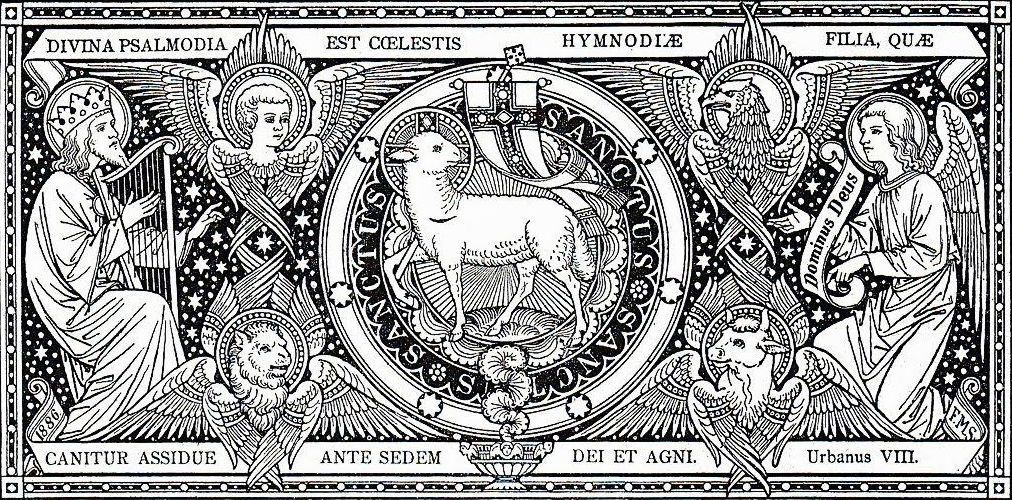
\includegraphics[width=1.0\textwidth]{divina_psalmodia.jpg}
	\vfill
	\fontspec{jsl-ancient.ttf}
	\fontsize{46}{50}\selectfont
	{Hymny laudesowe}\par
	\normalfont
	\vfill
	
\includegraphics[width=0.6\textwidth]{benedicamus_domino.jpg}
\end{center}

%% -----------------  SPIS TREŚCI ---------------------
\tableofcontents
\pagenumbering{arabic}

%% -----------------  HYMNY ORDINARIUM DIVINI PFFICII ET PSALTERIUM ---------------------
\part{PSALTERIUM}\setcounter{chapter}{0} % Zerowanie licznika rozdziałów
%% -----------------  HYMNY Dominica   ---------------------
\chapter{Dominica}
\section{Ecce jam noctis tenuatur} \index{Ecce jam noctis tenuatur}
\begin{center}
	\noindent\small\textit{Liber antiphonarius, Solesmes, 1960, p.9}
\end{center}	
\vspace{5mm}
\begin{paracol}{2}
	\ensurevspace{4cm}
	\begin{nutybox}
	\greannotation{Hymn.} \greannotation{1.} \gabcsnippet{(c4) EC(d)ce(c') jam(d) no(fg)ctis(f.) (,) te(g')nu(h)á(g')tur(f) um(g)bra,(h.) (;) Lux(gh) et(i) au(h')ró(g)rae(fe) rú(d')ti(f)lans(e') co(f)rú(d)scat:(c.) (:) Súp(d)pli(c')ces(d) re(fg)rum(f.) (,) Dó(g')mi(h)num(g') ca(f)nó(e)ra(d.) (,) Vo(f)ce(e') pre(f)cé(dc)mur:(d.) (::)}
	\end{nutybox}
	\switchcolumn
	\begin{tlumbox}
	\vspace{3.5mm} 
	\red{1.} Oto już niknie cień nocy, i\,światło jutrzenki jaśnieje różowo: wdzięcznym głosem módlmy się kornie do Pana (wszech)rzeczy:\end{tlumbox}
  	\ensurevspace{4cm}
	\switchcolumn*
	\begin{nutybox}
	\gresetinitiallines{0}\gabcsnippet{(c4) <c>2.</c> Ut(d) re(c')os(d) cul(fg)pae(f.) (,) mi(g')se(h)rá(g')tus,(f) o(g)mnem(h.) (;) Pel(gh)lat(i) an(h')gó(g)rem(fe) trí(d')bu(f)at(e') sa(f)lú(d)tem,(c.) (:) Do(d)net(c') et(d) no(fg)bis(f.) (,) bo(g')na(h) sem(g')pi(f)tér(e)nae(d.) (,) Mú(f)ne(e')ra(f) pa(dc)cis.(d.) (::)}
	\end{nutybox}
	\switchcolumn
	\begin{tlumbox}
	\vspace{3.5mm} 
	\red{2.} Iżby, litując się nad obarczony mi winą, oddalił wszelki lęk, udzielił zbawienia i\,dał nam dobre dary pokoju wiekuistego.
	\end{tlumbox}
	\ensurevspace{4cm}
	\switchcolumn*
	\begin{nutybox}
	\gresetinitiallines{0}\gabcsnippet{(c4) <c>3.</c> Prae(d)stet(c') hoc(d) no(fg)bis(f.) (,) Dé(g')i(h)tas(g') be(f)á(g)ta(h.) (;) Pa(gh)tris,(i) ac(h') Na(g)ti,(fe) pa(d')ri(f)tér(e')que(f) San(d)cti(c.) (:) Spí(d)ri(c')tus,(d) cu(fg)jus(f.) (,) ré(g')so(h)nat(g') per(f) o(e)mnem(d.) (,) Gló(f)ri(e')a(f) mun(dc)dum.(d.) (::) A(ded)men.(cd..) (::)}
	\end{nutybox}
	\switchcolumn
	\begin{tlumbox}
	\vspace{3.5mm} 
	\red{3.} Niechaj nam tego użyczy błogosławione Bóstwo Ojca i\,Syna, jako też Ducha Świętego, którego chwała po całym rozbrzmiewa świecie.
	\end{tlumbox}
\end{paracol}	
\koniec		
%% -----------------
\section{Aeterne rerum} \index{Aeterne rerum}
\begin{center}
	\noindent\small\textit{Antiphonale Monasticum, Solesmes, 1934, p.34}
\end{center}	
\vspace{5mm}
\begin{paracol}{2}
	\ensurevspace{4cm}
	\begin{nutybox}\greannotation{Hymn.} \greannotation{1.} \gabcsnippet{(c4)Æ(f)tér(f')ne(g) re(h)rum(ixi) Cón(h')di(g)tor,(h'_) (,)Noc(h)tem(g') di(j)ém(j)que(g) qui(h') re(ixi)gis,(h.) (;)Et(g) tém(h')po(g)rum(h) das(g) tém(e')po(f)ra,(g'_) (,)Ut(g) ál(h')le(g)ves(f) fas(e)tí(fg)di(fe)um(d.) (::)}
	\end{nutybox}
	\switchcolumn
	\begin{tlumbox}
	\vspace{3.5mm} 
	Wieczysty Stwórco świata, Władco nocy i\,świtu, Co czas urozmaicasz, By strzec nas od przesytu.
	\end{tlumbox}
  	\ensurevspace{4cm}
	\switchcolumn*
	\begin{nutybox}
	\gresetinitiallines{0}\gabcsnippet{(c4) 2A. Præ(f)co(f') di(g)é(h)i(ixi) iam(h') so(g)nat,(h'_) (,) Noc(h)tis(g') pro(j)fún(j)dæ(g) pér(h')vi(ixi)gil,(h.) (;) Noc(g)túr(h')na(g) lux(h) vi(g)án(e')ti(f)bus(g'_) (,) A(g) noc(h')te(g) noc(f)tem(e) sé(fg)gre(fe)gans.(d.) (::)}
	\end{nutybox}
	\switchcolumn
	\begin{tlumbox}
	\vspace{3.5mm} 
	Już pieje dnia radosny zwiastun, Który w\,głębokiej nocy czuwa. Światło wśród mroku dla wędrowców, Światło dzielące noc od nocy. \end{tlumbox}
  	\ensurevspace{4cm}
	\switchcolumn*
	\begin{nutybox}
	\gresetinitiallines{0}\gabcsnippet{(c4) 2B. Præ(f)co(f') di(g)é(h)i(ixi) iam(h') so(g)nat,(h'_) (,) Noc(h)tis(g') pro(j)fún(j)dæ(g) pér(h')vi(ixi)gil,(h.) (;) Noc(g)túr(h')na(g) lux(h) vi(g)án(e')ti(f)bus(g'_) (,) A(g) noc(h')te(g) noc(f)tem(e) sé(fg)gre(fe)gans.(d.) (::)}
	\end{nutybox}
	\switchcolumn
	\begin{tlumbox}
	\vspace{3.5mm} 
	Wedrowców światło nocne, Co dzieli noc na straże, Kur, zwiastun dnia, się głosi i\,słońcu błysnąć każe.
	\end{tlumbox}
	\ensurevspace{4cm}
	\switchcolumn*
	\begin{nutybox}
	\gresetinitiallines{0}\gabcsnippet{(c4) <c>3.</c> Hoc(f) ex(f')ci(g)tá(h)tus(ixi) Lú(h')ci(g)fer(h'_) (,) Sol(h)vit(g') po(j)lum(j) ca(g)lí(h')gi(ixi)ne:(h.) (;)bHoc(g) om(h')nis(g) er(h)ró(g)num(e') co(f)hors(g'_) (,) Vi(g)am(h') no(g)cén(f)di(e) dé(fg)se(fe)rit.(d.) (::)}
	\end{nutybox}
	\switchcolumn
	\begin{tlumbox}
	\vspace{3.5mm} 
	Zbudzona z\,snu Jutrzenka Rozprasza mroku ślady i\,cały tłum złych duchów Opuszcza drogę zdrady.
	\end{tlumbox}
	\ensurevspace{4cm}
	\switchcolumn*
	\begin{nutybox}
	\gresetinitiallines{0}\gabcsnippet{(c4) <c>4.</c> Hoc(f) nau(f')ta(g) vi(h)res(ixi) cól(h')li(g)git,(h'_) (,) Pon(h)tí(g')que(j) mi(j)tés(g)cunt(h') fre(ixi)ta:(h.) (;) Hoc,(g) ip(h')sa(g) pe(h)tr<i>a</i>() Ec(g)clé(e')si(f)æ,(g'_) (,) Ca(g)nén(h')te,(g) cul(f)pam(e) dí(fg)lu(fe)it.(d.) (::)}
	\end{nutybox}
	\switchcolumn
	\begin{tlumbox}
	\vspace{3.5mm} 
	Żeglarz znów zbiera siły i\,cichną mórz głębiny, Nawet Kościoła skała Kaja się swojej winy.
	\end{tlumbox}
	\ensurevspace{4cm}
	\switchcolumn*
	\begin{nutybox}
	\gresetinitiallines{0}\gabcsnippet{(c4) <c>5.</c> Sur(f)gá(f')mus(g) er(h)go(ixi) stré(h')nu(g)e:(h'_) (,) Gal(h)lus(g') ja(j)cén(j)tes(g) éx(h')ci(ixi)tat,(h.) (;) Et(g) som(h')no(g)lén(h)tos(g) ín(e')cre(f)pat,(g'_) (,)  Gal(g)lus(h') ne(g)gán(f)tes(e) ár(fg)gu(fe)it.(d.) (::)}
	\end{nutybox}
	\switchcolumn
	\begin{tlumbox}
	\vspace{3.5mm} 
	Wstawajcie tedy szybko! Kur wczasujących budzi, w\,śnie pogrążonych gani, Oskarża gnuśnych ludzi.
	\end{tlumbox}
	\ensurevspace{4cm}
	\switchcolumn*
	\begin{nutybox}
	\gresetinitiallines{0}\gabcsnippet{(c4) <c>6.</c> Gal(f)lo(f') ca(g)nén(h)te,(ixi) spes(h') red(g)it,(h'_) (,) Æ(h)gris(g') sa(j)lus(j) re(g)fún(h')di(ixi)tur,(h.) (;) Mu(g)cro(h') la(g)tró(h)nis(g) cón(e')di(f)tur,(g'_) (,) Lap(g)sis(h') fi(g)des(f) re(e)vér(fg)ti(fe)tur.(d.) (::)}
	\end{nutybox}
	\switchcolumn
	\begin{tlumbox}
	\vspace{3.5mm} 
	Pianiem nadzieję wskrzesza Chory się czuje lepiej, Zbój miecz do pochwy chowa, w\,upadłych wiarę krzepi.
	\end{tlumbox}
	\ensurevspace{4cm}
	\switchcolumn*
	\begin{nutybox}
	\gresetinitiallines{0}\gabcsnippet{(c4) <c>7.</c> Je(f)su,(f') la(g)bén(h)tes(ixi) ré(h')spi(g)ce,(h'_) (,) Et(h) nos(g') vi(j)dén(j)do(g) cór(h')ri(ixi)ge:(h.) (;) Si(g) ré(h')spi(g)cis,(h) lap(g)si(e') sta(f)bunt,(g'_) (,) Fle(g)tú(h')que(g) cul(f)pa(e) sól(fg)vi(fe)tur.(d.) (::)}
	\end{nutybox}
	\switchcolumn
	\begin{tlumbox}
	\vspace{3.5mm} 
	Wejrz, Jezu, na upadłych, Podnieś ich swym spojrzeniem: Gdy spojrzysz, giną grzechy Obmyte łez strumieniem.
	\end{tlumbox}
	\ensurevspace{4cm}
	\switchcolumn*
	\begin{nutybox}
	\gresetinitiallines{0}\gabcsnippet{(c4) <c>8.</c> Tu,(f) lux,(f') re(g)fúl(h)ge(ixi) sén(h')si(g)bus,(h'_) (,) Men(h)tís(g')que(j) som(j)num(g) dís(h')cu(ixi)te:(h.) (;) Te(g) nos(h')tra(g) vox(h) pri(g)mum(e') so(f)net,(g'_) (,) Et(g) vo(h')ta(g) sol(f)vá(e)mus(fg) ti(fe)bi.(d.) (::)}
	\end{nutybox}
	\switchcolumn
	\begin{tlumbox}
	\vspace{3.5mm} 
	O światło, błyśnij sercem, Wypłosz z\,dusz snu omamy: Nad wszystko Cię sławimy i\,ślubów dotrzymamy.
	\end{tlumbox}
	\ensurevspace{4cm}
	\switchcolumn*
	\begin{nutybox}
	\gresetinitiallines{0}\gabcsnippet{(c4) <c>9.</c> De(f)o(f') Pa(g)tri(h) sit(ixi) gló(h')ri(g)a,(h'_) (,) E(h)iús(g')que(j) so(j)li(g) Fí(h')li(ixi)o,(h.) (;) Cum(g) Spí(h')ri(g)tu(h) Pa(g)rá(e')cli(f)to,(g'_) (,) Et(g) nunc,(h') et(g) in(f) per(e)pé(fg)tu(fe)um.(d.) (::) A(ded)men.(cd..) (::)}
	\end{nutybox}
	\switchcolumn
	\begin{tlumbox}
	\vspace{3.5mm} 
	Więc chwalmy Boga Ojca i\,Syna Jedynego z\,Duchem Pocieszycielem Na wieki, dnia każdego.\footnotemark
	\end{tlumbox}
	\footnotetext{tłum. L.Staff oprócz 2B - tłum. Z.Kubiak} 
\end{paracol}	
\koniec		
%% -----------------  HYMNY Feria Secunda ---------------------
\chapter{Feria Secunda}
\section{Splendor paternae gloriae} \index{Splendor paternae gloriae}
\begin{center}
	\textit{Antiphonale Monasticum, Solesmes, 1934, p. 44}
\end{center}	
\vspace{5mm}
\begin{paracol}{2}
	\ensurevspace{4cm}
	\begin{nutybox}\greannotation{Hymn.} \gabcsnippet{(c4)Splen(e)dor(c) pa(d')tér(f)næ,(ef) gló(g')ri(f)æ,(e.)  (,)De(e) lu(c)ce(d') lu(f)cem(ef) pró(g')fe(g)rens,(g.) (;)Lux(g) lu(f)cis,(g') et(h) fons(gf) lú(g')mi(f)nis,(e.) (,)Di(e)em(c) di(d')es(f) il(ef)lú(g')mi(f)nans:(e.) (::)}
	\end{nutybox}
	\switchcolumn
	\begin{tlumbox}
	\vspace{3.5mm} 
	Blasku chwały Ojcowskiej, z\,światłości przynoszący światłość, światło światłości i\,źródło jasności, dniem dzień oświetlający:\end{tlumbox}
  	\ensurevspace{4cm}
	\switchcolumn*
	\begin{nutybox}
	\gresetinitiallines{0}\gabcsnippet{(c4) <c>2.</c> Ve(e)rús(c)que(d') sol(f) il(ef)lá(g')be(f)re,(e.) (,) Mi(e)cans(c) ni(d')tó(f)re(ef) pér(g')pe(g)ti:(g.) (;) Ju(g)bár(f)que(g') San(h)cti(gf) Spí(g')ri(f)tus(e.) (,) In(e)fún(c)de(d') no(f)stris(ef) sén(g')si(f)bus.(e.) (::)}
	\end{nutybox}
	\switchcolumn
	\begin{tlumbox}
	\vspace{3.5mm} 
	i\,spuść się jako słońce prawdziwe, jaśniejące blaskiem niegasnącym: i\,światło Ducha Świętego wlej do serc naszych.
	\end{tlumbox}
	\ensurevspace{4cm}
	\switchcolumn*
	\begin{nutybox}
	\gresetinitiallines{0}\gabcsnippet{(c4) <c>3.</c> Vo(e)tis(c) vo(d')cé(f)mus(ef) et(g') Pa(f)trem,(e.) (,) Pa(e)trem(c) pe(d')rén(f)nis(ef) gló(g')ri(g)æ,(g.) (;) Pa(g)trem(f) po(g')tén(h)tis(gf) grá(g')ti(f)æ,(e.) (,) Cul(e)pam(c) re(d')lé(f)get(ef) lú(g')bri(f)cam.(e.) (::)}
	\end{nutybox}
	\switchcolumn
	\begin{tlumbox}
	\vspace{3.5mm} 
	Prośbami wołajmy także do Ojca, Ojca możnej łaski, Ojca wiecznej chwały, aby oddalał (od nas) winę zgubną.
	\end{tlumbox}
	\ensurevspace{4cm}
	\switchcolumn*
	\begin{nutybox}
	\gresetinitiallines{0}\gabcsnippet{(c4) <c>4.</c> Con(e)fír(c)met(d') a(f)ctus(ef) stré(g')nu(f)os,(e.) (,) Den(e)tes(c) re(d')tún(f)dat(ef) ín(g')vi(g)di,(g.) (;) Ca(g)sus(f) se(g')cún(h)det(gf) á(g')spe(f)ros,(e.) (,) Do(e)net(c) ge(d')rén(f)di(ef) grá(g')ti(f)am.(e.) (::)}
	\end{nutybox}
	\switchcolumn
	\begin{tlumbox}
	\vspace{3.5mm} 
	Niechaj utwierdzi czyny stanowcze, zęby stępi zawistnika, sprzyja w\,wypadkach przykrych, (tem, co) czynić trzeba, kieruje należycie.
	\end{tlumbox}
	\ensurevspace{4cm}
	\switchcolumn*
	\begin{nutybox}
	\gresetinitiallines{0}\gabcsnippet{(c4) <c>5.</c> Men(e)tem(c) gu(d')bér(f)net(ef) et(g') re(f)gat,(e.) (,) Ca(e)sto,(c) fi(d')dé(f)li(ef) cór(g')po(g)re;(g.) (;) Fi(g)des(f) ca(g')ló(h)re(gf) fér(g')ve(f)at,(e.) (,) Frau(e)dis(c) ve(d')né(f)na(ef) né(g')sci(f)at.(e.) (::)}
	\end{nutybox}
	\switchcolumn
	\begin{tlumbox}
	\vspace{3.5mm} 
	Ducha niechaj wiedzie i\,(nim) kieruje; niech czystość nasza pozostanie nieskalana, wiara niechaj pała żarem i\,nie zna jadu fałszu.
	\end{tlumbox}
	\ensurevspace{4cm}
	\switchcolumn*
	\begin{nutybox}
	\gresetinitiallines{0}\gabcsnippet{(c4) <c>6.</c> Chri(e)stús(c)que(d') no(f)bis(ef) sit(g') ci(f)bus,(e.) (,) Po(e)tús(c)que(d') no(f)ster(ef) sit(g') fi(g)des:(g.) (;) Læ(g)ti(f) bi(g')bá(h)mus(gf) só(g')bri(f)am(e.) (,) E(e)bri(c)e(d')tá(f)tem(ef) Spí(g')ri(f)tus.(e.) (::)}
	\end{nutybox}
	\switchcolumn
	\begin{tlumbox}
	\vspace{3.5mm} 
	Chrystus też niechaj będzie naszym pokarmem, a wiara naszym napojem; radośnie pijmy z\,nieupajającej obfitości Ducha (Św.).
	\end{tlumbox}
	\ensurevspace{4cm}
	\switchcolumn*
	\begin{nutybox}
	\gresetinitiallines{0}\gabcsnippet{(c4) <c>7.</c> Læ(e)tus(c) di(d')es(f) hic(ef) trán(g')se(f)at,(e.) (,) Pu(e)dor(c) sit(d') ut(f) di(ef)lú(g')cu(g)lum,(g.) (;) Fi(g)des(f) ve(g')lut(h) me(gf)rí(g')di(f)es,(e.) (,) Cre(e)pú(c)scu(d')lum(f) mens(ef) né(g')sci(f)at.(e.) (::)}
	\end{nutybox}
	\switchcolumn
	\begin{tlumbox}
	\vspace{3.5mm} 
	Niechaj dzień ten przejdzie radośnie, wstydliwość niechaj będzie jako świt, wiara jako południe, zmroku niechaj duch nie zazna.
	\end{tlumbox}
	\ensurevspace{4cm}
	\switchcolumn*
	\begin{nutybox}
	\gresetinitiallines{0}\gabcsnippet{(c4) <c>8.</c> Au(e)ró(c)ra(d') cur(f)sus(ef) pró(g')ve(f)hit,(e.) (,) Au(e)ró(c)ra(d') to(f)tus(ef) pró(g')de(g)at,(g.) (;) In(g) Pa(f)tre(g') to(h)tus(gf) Fí(g')li(f)us,(e.) (,) Et(e) to(c)tus(d') in(f) Ver(ef)bo(g') Pa(f)ter.(e.) (::)}
	\end{nutybox}
	\switchcolumn
	\begin{tlumbox}
	\vspace{3.5mm} 
	Jutrzenka sprowadza światło, z\,światłem (zaś) niechaj nam objawi się w\,Ojcu Syn cały i\,cały w\,Słowie Ojciec.
	\end{tlumbox}
	\ensurevspace{4cm}
	\switchcolumn*
	\begin{nutybox}
	\gresetinitiallines{0}\gabcsnippet{(c4) <c>9.</c> De(e)o(c) Pa(d')tri(f) sit(ef) gló(g')ri(f)a,(e.) (,) E(e)jús(c)que(d') so(f)li(ef) Fí(g')li(g)o,(g.) (;) Cum(g) Spí(f)ri(g')tu(h) Pa(gf)rá(g')cli(f)to,(e.) (,) Et(e) nunc,(c) et(d') in(f) per(ef)pé(g')tu(f)um.(e.) (::) A(efe)men.(de..) (::)}
	\end{nutybox}
	\switchcolumn
	\begin{tlumbox}
	\vspace{3.5mm} 
	Bogu Ojcu niechaj będzie chwała i\,jedynemu jego Synowi wraz z\,Duchem Pocieszycielem teraz i\,po wszystek wiek. Amen.
	\end{tlumbox}
\end{paracol}	
\koniec		

%% -----------------  HYMNY ---------------------
\chapter{Feria Tertia}
\section{Ales diei nuntius} \index{Ales diei nuntius}
\begin{center}
	\noindent\small\textit{Liber antiphonarius, Solesmes, 1960, p.109}
\end{center}	
\vspace{5mm}
\begin{paracol}{2}
	\ensurevspace{4cm}
	\begin{nutybox}\greannotation{Hymn.} \greannotation{4.} \gabcsnippet{(c4) A(e)les(c') di(d)é(f)i(ef) nún(g')ti(f)us(e) (,) Lu(e)cem(c') pro(d)pín(f)quam(ef) praé(g')ci(g)nit:(g.) (;) Nos(g) ex(g')ci(h)tá(h)tor(f) mén(g')ti(f)um,(e) (,) Jam(e) Chri(c')stus(d) ad(f) vi(ef)tam(g') vo(f)cat.(e.) (::)}
	\end{nutybox}
	\switchcolumn
	\begin{tlumbox}
	\vspace{3.5mm} 
	Skrzydlaty zwiastun dnia Zapowiada bliski świt: Wskrzesiciel duchów Chrystus Już nas powołuje do życia.
	\end{tlumbox}
  	\ensurevspace{4cm}
	\switchcolumn*
	\begin{nutybox}
	\gresetinitiallines{0}\gabcsnippet{(c4) <c>2.</c> Au(e)fér(c')te,(d) cla(f)mat(ef) lé(g')ctu(f)los,(e) (,) Æ(e)gro(c') so(d)pó(f)re(ef) dé(g')si(g)des:(g.) (;) Ca(g)stí(g')que,(h) re(h)ct<i>i</i>() ac(f) só(g')bri(f)i(e) (,) Vi(e)g<i>i</i>()lá(c')te:(d) jam(f) sum(ef) pró(g')xi(f)mus.(e.) (::)}
	\end{nutybox}
	\switchcolumn
	\begin{tlumbox}
	\vspace{3.5mm} 
	Ociężali od snu gnuśnego, Odsuńcie — woła — łoża, Czyści, prawi i\,trzeźwi Czuwajcie, już jestem bliski.
	\end{tlumbox}
	\ensurevspace{4cm}
	\switchcolumn*
	\begin{nutybox}
	\gresetinitiallines{0}\gabcsnippet{(c4) <c>3.</c> Je(e)sum(c') ci(d)á(f)mus(ef) vó(g')ci(f)bus,(e) (,) Flen(e)tes,(c') pre(d)cán(f)tes,(ef) só(g')bri(g)i:(g.) (;) In(g)tén(g')ta(h) sup(h)pli(f)cá(g')ti(f)o(e) (,) Dor(e)mí(c')re(d) cor(f) mun(ef)dum(g') ve(f)tat.(e.) (::)}
	\end{nutybox}
	\switchcolumn
	\begin{tlumbox}
	\vspace{3.5mm} 
	Jezusa przywołujmy głosami Płacząc, błagając trzeźwi: Niechaj żarliwa modlitwa Nie pozwala zasypiać sercu czystemu.
	\end{tlumbox}
	\ensurevspace{4cm}
	\switchcolumn*
	\begin{nutybox}
	\gresetinitiallines{0}\gabcsnippet{ (c4) <c>4.</c> Tu(e) Chri(c')ste(d) so(f)mnum(ef) dí(g')scu(f)te,(e) (,) Tu(e) rum(c')pe(d) no(f)ctis(ef) vín(g')cu(g)la,(g.) (;) Tu(g) sol(g')ve(h) pec(h)cá(f)tum(g') ve(f)tus,(e) (,) No(e)vúm(c')que(d) lu(f)men(ef) ín(g')ge(f)re.(e.) (::)}
	\end{nutybox}
	\switchcolumn
	\begin{tlumbox}
	\vspace{3.5mm} 
	Ty, Chryste, rozprosz sen, Ty skrusz więzy nocy, Ty rozwiąż grzech, A wznieś światło nowe.
	\end{tlumbox}
	\ensurevspace{4cm}
	\switchcolumn*
	\begin{nutybox}
	\gresetinitiallines{0}\gabcsnippet{(c4) <c>5.</c> De(e)o(c') Pa(d)tri(f) sit(ef) gló(g')ri(f)a,(e) (,) E(e)jú(c')sque(d) so(f)li(ef) Fí(g')li(g)o,(g.) (;) Cum(g) Spí(g')ri(h)tu(h) Pa(f)rá(g')cli(f)to,(e) (,) Nunc(e) et(c') per(d) o(f)mne(ef) saé(g')cu(f)lum.(e.) (::) A(efe)men.(de..) (::)}
	\end{nutybox}
	\switchcolumn
	\begin{tlumbox}
	\vspace{3.5mm} 
	Bogu Ojcu niechaj będzie chwała i\,jedynemu Jego Synowi Wraz z\,Duchem Pocieszycielem Teraz i\,po wszystek wiek. Amen.
	\end{tlumbox}
\end{paracol}	
\koniec		

%% -----------------  HYMNY Feria Quarta ---------------------
\section{Nox et tenebrae (hiemalis, mod.1)} \index{Nox et tenebrae (hiemalis, mod.1)}
\begin{center}
	\noindent\small\textit{Antiphonale Monasticum, Solesmes, 1934, p.57}
\end{center}	
\vspace{5mm}
\begin{paracol}{2}
	\ensurevspace{4cm}
	\begin{nutybox}\greannotation{Hymn.} \greannotation{1.} \gabcsnippet{(c4)NOX,(h) et(h') te(h)né(h)br<i>æ</i>,() et(h) nú(hi)bi(h)la,(h'_) (,)Con(h)fú(h')sa(h) mun(g)d<i>i</i>() et(f) túr(gh)bi(g)da;(g.) (;)Lux(f) int(h')rat,(h) al(g)bés(f)cit(g') po(g)lus :(h'_) (,)Chris(g)tus(g') ve(g)nit,(f) dis(d)cé(f')di(e)te.(d.) (::)}
	\end{nutybox}
	\switchcolumn
	\begin{tlumbox}
	\vspace{3.5mm} 
	Noc, i\,ciemności, i\,chmury, (wszystko cokolwiek) na świecie (jest) zmieszanego i\,wzburzonego, ustąpcie: Światło wschodzi, rozjaśnia się niebo: Chrystus idzie.
	\end{tlumbox}
  	\ensurevspace{4cm}
	\switchcolumn*
	\begin{nutybox}
	\gresetinitiallines{0}\gabcsnippet{(c4) <c>2.</c> Ca(h)lí(h')go(h) ter(h)ræ(h) scín(hi)di(h)tur(h'_) (,) Per(h)cús(h')sa(h) so(g)lis(f) spí(gh)cu(g)lo,(g.) (;) Re(f)bús(h')que(h) iam(g) co(f)lor(g') red(g)it,(h'_) (,) Vul(g)tu(g') ni(g)tén(f)tis(d) sí(f')de(e)ris.(d.) (::)}
	\end{nutybox}
	\switchcolumn
	\begin{tlumbox}
	\vspace{3.5mm} 
	Ciemność na ziemi przerywa się, Prażona ostrzem słońca, i\,wraca już rzeczom barwność (ich) Na widok jaśniejącego słońca.
	\end{tlumbox}
	\ensurevspace{4cm}
	\switchcolumn*
	\begin{nutybox}
	\gresetinitiallines{0}\gabcsnippet{(c4) <c>3.</c> Te,(h) Chris(h')te,(h) so(h)lum(h) nó(hi)vi(h)mus:(h'_) (,) Te(h) men(h')te(h) pu(g)r<i>a</i>() et(f) sím(gh)pli(g)ci,(g.) (;) Flen(f)d<i>o</i>() et(h') ca(h)nén(g)do(f) quǽ(g')su(g)mus,(h'_) (,) In(g)tén(g')de(g) nos(f)tris(d) sén(f')si(e)bus.(d.) (::)}
	\end{nutybox}
	\switchcolumn
	\begin{tlumbox}
	\vspace{3.5mm} 
	Ciebie, Chryste, jedynego znamy: Ciebie sercem czystem i\,prostem, Płacząc i\,śpiewając, prosimy, Zwróć się ku naszej duszy.
	\end{tlumbox}
	\ensurevspace{4cm}
	\switchcolumn*
	\begin{nutybox}
	\gresetinitiallines{0}\gabcsnippet{(c4) <c>4.</c> Sunt(h) mul(h')ta(h) fu(h)cis(h) íl(hi)li(h)ta,(h'_) (,) Quæ(h) lu(h')ce(h) pur(g)gén(f)tur(gh) tu(g)a:(g.) (;) Tu,(f) lux(h') E(h)ó(g)i(f) sí(g')de(g)ris,(h'_) (,) Vul(g)tu(g') se(g)ré(f)n<i>o</i>() il(d)lú(f')mi(e)na.(d.) (::)}
	\end{nutybox}
	\switchcolumn
	\begin{tlumbox}
	\vspace{3.5mm} 
	Dużo jest (rzeczy) pokrytych fałszywemi barwami, Które oczyszcza światło twoje: Ty, prawdziwa światłości niebian, Oświeć (nas) pogodnem wejrzeniem.
	\end{tlumbox}
	\ensurevspace{4cm}
	\switchcolumn*
	\begin{nutybox}
	\gresetinitiallines{0}\gabcsnippet{(c4) <c>5.</c> De(h)o(h') Pa(h)tri(h) sit(h) gló(hi)ri(h)a,(h'_) (,) E(h)iús(h')que(h) so(g)li(f) Fí(gh)li(g)o,(g.) (;) Cum(f) Spí(h')ri(h)tu(g) Pa(f)rá(g')cli(g)to,(h'_) (,) Et(g) nunc,(g') et(g) in(f) per(d)pé(f')tu(e)um.(d.) (::) A(ded)men.(cd..) (::)}
	\end{nutybox}
	\switchcolumn
	\begin{tlumbox}
	\vspace{3.5mm} 
	Bogu Ojcu niechaj będzie chwała i\,jedynemu Jego Synowi Wraz z\,Duchem Pocieszycielem Teraz i\,po wszystek wiek. Amen.\footnotemark
	\end{tlumbox}
	\footnotetext{tłum. Ks. Bronisław Gładysz, "Hymny brewiarza rzymskiego oraz patronału polskiego. Przekład i objaśnienia", Poznań 1933} 
\end{paracol}	
\koniec		

%% ----------------- HYMNY -----------------
\chapter{Feria Quarta}
\section{Nox et tenebrae (aestivalis, mod.4)} \index{Nox et tenebrae (aestivalis, mod.4)}
\begin{center}
	\noindent\small\textit{Antiphonale Monasticum, Solesmes, 1934, p.57}
\end{center}	
\vspace{5mm}
\begin{paracol}{2}
	\ensurevspace{4cm}
	\begin{nutybox}\greannotation{Hymn.} \greannotation{4.} \gabcsnippet{(c4) NOX,(e) et(c') te(d)né(f)br<i>ae</i>,() et(ef) nú(g')bi(f)la,(e) (,) Con(e)fú(c')sa(d) mun(f)d<i>i</i>() et(ef) túr(g')bi(g)da:(g.) (;) Lux(g) in(g')trat,(h) al(h)bé(f)scit(g') po(f)lus:(e) (,) Chri(e)stus(c') ve(d)nit,(f) di(ef)scé(g')di(f)te.(e.) (::)}
	\end{nutybox}
	\switchcolumn
	\begin{tlumbox}
	\vspace{3.5mm} 
	Noc, i\,ciemności, i\,chmury, Wszystko cokolwiek na świecie Zmieszanego i\,wzruszonego, ustąpcie: Światło wschodzi, rozjaśnia się niebo: Chrystus idzie.
	\end{tlumbox}
  	\ensurevspace{4cm}
	\switchcolumn*
	\begin{nutybox}
	\gresetinitiallines{0}\gabcsnippet{(c4) <c>2.</c> Ca(e)lí(c')go(d) ter(f)rae(ef) scín(g')di(f)tur,(e) (,) Per(e)cús(c')sa(d) so(f)lis(ef) spí(g')cu(g)lo:(g.) (;) Re(g)bú(g')sque(h) jam(h) co(f)lor(g') re(f)dit(e) (,) Vul(e)tu(c') ni(d)tén(f)tis(ef) sí(g')de(f)ris.(e.) (::)}
	\end{nutybox}
	\switchcolumn
	\begin{tlumbox}
	\vspace{3.5mm} 
	Ciemność na ziemi przerywa się, Prażona ostrzem słońca, i\,wraca już rzeczom barwność Na widok jaśniejącego słońca.
	\end{tlumbox}
	\ensurevspace{4cm}
	\switchcolumn*
	\begin{nutybox}
	\gresetinitiallines{0}\gabcsnippet{(c4) <c>3.</c> Te(e) Chri(c')ste(d) so(f)lum(ef) nó(g')vi(f)mus,(e) (,) Te(e) men(c')te(d) pu(f)r<i>a</i>() et(ef) sím(g')pli(g)ci,(g.) (;) Flen(g)d<i>o</i>() et(g') ca(h)nén(h)do(f) quaé(g')su(f)mus,(e) (,) In(e)tén(c')de(d) no(f)stris(ef) sén(g')si(f)bus.(e.)(::)}
	\end{nutybox}
	\switchcolumn
	\begin{tlumbox}
	\vspace{3.5mm} 
	Ciebie, Chryste, jedynego znamy: Ciebie sercem czystem i\,prostem, Płacząc i\,śpiewając, prosimy, Zwróć się ku naszej duszy.
	\end{tlumbox}
	\ensurevspace{4cm}
	\switchcolumn*
	\begin{nutybox}
	\gresetinitiallines{0}\gabcsnippet{(c4) <c>4.</c> Sunt(e) mul(c')ta(d) fu(f)cis(ef) íl(g')li(f)ta,(e) (,) Quae(e) lu(c')ce(d) pur(f)gén(ef)tur(g') tu(g)a:(g.) (;) Tu(g) ve(g')ra(h) lux(h) cae(f)lé(g')sti(f)um(e) (,) Vul(e)tu(c') se(d)ré(f)n<i>o</i>() il(ef)lú(g')mi(f)na.(e.) (::)}
	\end{nutybox}
	\switchcolumn
	\begin{tlumbox}
	\vspace{3.5mm} 
	Dużo jest pokrytych fałszywemi barwami, Które oczyszcza światło twoja: Ty, prawdziwa światłości niebian, Oświeć nas pogodnem wejrzeniem.
	\end{tlumbox}
	\ensurevspace{4cm}
	\switchcolumn*
	\begin{nutybox}
	\gresetinitiallines{0}\gabcsnippet{(c4) 5.(::) De(e)o(c') Pa(d)tri(f) sit(ef) gló(g')ri(f)a,(e) (,) E(e)jú(c')sque(d) so(f)li(ef) Fí(g')li(g)o,(g.) (;) Cum(g) Spí(g')ri(h)tu(h) Pa(f)rá(g')cli(f)to,(e) (,) Nunc(e) et(c') per(d) o(f)mne(ef) saé(g')cu(f)lum.(e.) (::) A(efe)men.(de..) (::)}
	\end{nutybox}
	\switchcolumn
	\begin{tlumbox}
	\vspace{3.5mm} 
	Bogu Ojcu niechaj będzie chwała i\,jedynemu Jego Synowi Wraz z\,Duchem Pocieszycielem Teraz i\,po wszystek wiek. Amen.
	\end{tlumbox}
\end{paracol}	
\koniec		

%% -----------------  HYMNY Feria Quinta ---------------------
% Lux ecce surgit (1.) - in Hieme
\chapter{Feria Quinta}
\section{Lux ecce surgit} \index{Lux ecce surgit}
\begin{center}
	\noindent\small\textit{Antiphonale Monasticum, Solesmes, 1934, p.65}
\end{center}	
\vspace{5mm}
\begin{paracol}{2}
	\ensurevspace{4cm}
	\begin{nutybox}\greannotation{Hymn.} \greannotation{4.} \gabcsnippet{(c4) LUX(e) ec(c)ce(d') sur(f)git(ef) áu(g')re(f)a,(e.) (,)Pal(e)lens(c) fa(d')tís(f)cat(ef) cǽ(g')ci(g)tas,(g.) (;)Quæ(g) nos(f)met(g') in(h) præ(gf)ceps(g') di(f)u(e.) (,)Er(e)ró(c)re(d') tra(f)xit(ef) dé(g')vi(f)o.(e.) (::)}
	\end{nutybox}
	\switchcolumn
	\begin{tlumbox}
	\vspace{3.5mm} 
	Oto światło powstaje złociste, Blednąc niechaj odejdzie ciemność, Która długo nas ciągnęła w\,przepaść omamieniem zdrożnem.
	\end{tlumbox}
  	\ensurevspace{4cm}
	\switchcolumn*
	\begin{nutybox}
	\gresetinitiallines{0}\gabcsnippet{ (c4) <c>2.</c> Hæc(e) lux(c) se(d')ré(f)num(ef) cón(g)fe(f)rat,(e.) (,)
Pu(e)rós(c)que(d') nos(f) præ(ef)stet(g) si(g)bi:(g.) (;)
Ni(g)hil(f) lo(g')quá(h)mur(gf) súb(g')do(f)lum:(e.) (,)
Vol(e)vá(c)mus(d') obs(f)cú(ef)rum(g') ni(f)hil.(e.) (::)}
	\end{nutybox}
	\switchcolumn
	\begin{tlumbox}
	\vspace{3.5mm} 
	Światło to niechaj sprowadzi pogodę i\,niechaj nas uczyni dla siebie czystymi: Nie mówmy nic podstępnego, Nie żywmy w\,sercu nic ponurego.
	\end{tlumbox}
	\ensurevspace{4cm}
	\switchcolumn*
	\begin{nutybox}
	\gresetinitiallines{0}\gabcsnippet{ (c4) <c>3.</c> Sic(e) to(c)ta(d') de(f)cúr(ef)rat(g) di(f)es,(e.) (,)
Ne(e) lin(c)gua(d') men(f)dax,(ef) ne(g) ma(g)nus(g.) (;)
O(g)c<i>u</i>()lí(f)ve(g') pec(h)cent(gf) lú(g')bri(f)ci,(e.) (,)
Ne(e) no(c)xa(d') cor(f)pus(ef) ín(g')qui(f)net.(e.) (::)}
	\end{nutybox}
	\switchcolumn
	\begin{tlumbox}
	\vspace{3.5mm} 
	Tak niechaj upłynie dzień cały, By ani język kłamliwy, ani ręce, Ani oczy ruchliwe nie zgrzeszyły, By grzech nie zbrukał ciała.
	\end{tlumbox}
	\ensurevspace{4cm}
	\switchcolumn*
	\begin{nutybox}
	\gresetinitiallines{0}\gabcsnippet{ (c4) <c>4.</c> Spe(e)c<i>u</i>()lá(c)tor(d') a(f)stat(ef) dé(g)su(f)per,(e.) (,)
Qui(e) nos(c) di(d')é(f)bus(ef) óm(g)ni(g)bus,(g.) (;)
Ac(g)tús(f)que(g') nos(h)tros(gf) pró(g')spi(f)cit(e.) (,)
A(e) lu(c)ce(d') pri(f)m<i>a</i>() in(ef) vés(g')pe(f)rum(e.) (::)}
	\end{nutybox}
	\switchcolumn
	\begin{tlumbox}
	\vspace{3.5mm} 
	Jest na wysokości badający, Który po wszystkie dni przygląda się Nam i\,uczynkom naszym Od pierwszego światła aż do wieczora\end{tlumbox}
	\ensurevspace{4cm}
	\switchcolumn*
	\begin{nutybox}
	\gresetinitiallines{0}\gabcsnippet{(c4)  <c>5.</c> De(e)o(c) Pa(d')tri(f) sit(ef) gló(g)ri(f)a,(e.) (,)
E(e)iús(c)que(d') so(f)li(ef) Fí(g)li(g)o,(g.) (;)
Cum(g) Spí(f)ri(g')tu(h) Pa(gf)rá(g')cli(f)to,(e.) (,)
Et(e) nunc,(c) et(d') in(f) per(ef)pé(g')tu(f)um.(e.) (::)
A(efe)men.(de..) (::)}
	\end{nutybox}
	\switchcolumn
	\begin{tlumbox}
	\vspace{3.5mm} 
	Bogu Ojcu niechaj będzie chwała i\,jedynemu Jego Synowi Wraz z\,Duchem Pocieszycielem Teraz i\,po wszystek wiek. Amen.
	\end{tlumbox}
\end{paracol}	
\koniec		

%% -----------------  HYMNY Feria Sexta ---------------------
% Aeterna caeli gloria (1.) - in Hieme
\chapter{Feria Sexta}
\section{Aeterna caeli gloria} \index{Aeterna caeli gloria}
\begin{center}
	\noindent\small\textit{Liber antiphonarius, Solesmes, 1960, p.168}
\end{center}	
\vspace{5mm}
\begin{paracol}{2}
	\ensurevspace{4cm}
	\begin{nutybox}\greannotation{Hymn.} \greannotation{4.} \gabcsnippet{(c4) AE(e)tér(c')na(d) cae(f)li(ef) gló(g')ri(f)a,(e) (,) Be(e)á(c')ta(d) spes(f) mor(ef)tá(g')li(g)um,(g.) (;) Sum(g)mi(g') To(h)nán(h)tis(f) U(g')ni(f)ce,(e) (,) Ca(e)staé(c')que(d) pro(f)les(ef) Vír(g')gi(f)nis:(e.) (::)}
	\end{nutybox}
	\switchcolumn
	\begin{tlumbox}
	\vspace{3.5mm} 
	Odwieczna nieba chwało, Błogosławiona nadziejo śmiertelnych, Jednorodzony Boga Najwyższego i\,potomku czystej Dziewicy:\end{tlumbox}
  	\ensurevspace{4cm}
	\switchcolumn*
	\begin{nutybox}
	\gresetinitiallines{0}\gabcsnippet{(c4) <c>2.</c> Da(e) déx(c')te(d)ram(f) sur(ef)gén(g')ti(f)bus,(e) (,) Ex(e)súr(c')gat(d) et(f) mens(ef) só(g')bri(g)a,(g.) (;) Fla(g)grans(g') et(h) in(h) lau(f)dem(g') De(f)i(e) (,) Gra(e)tes(c') re(d)pén(f)dat(ef) dé(g')bi(f)tas.(e.) (::)}
	\end{nutybox}
	\switchcolumn
	\begin{tlumbox}
	\vspace{3.5mm} 
	Podaj prawicę dźwigającym się, Niechaj powstanie także duch trzeźwy i\,z zapałem ku chwale Bożej Oddaje dzięki należne.
	\end{tlumbox}
	\ensurevspace{4cm}
	\switchcolumn*
	\begin{nutybox}
	\gresetinitiallines{0}\gabcsnippet{(c4) <c>3.</c> Or(e)tus(c') re(d)fúl(f)get(ef) Lú(g')ci(f)fer,(e) (,) Prae(e)ít(c')que(d) so(f)lem(ef) nún(g')ti(g)us:(g.) (;) Ca(g)dunt(g') te(h)né(h)brae(f) nó(g')cti(f)um,(e) (,) Lux(e) san(c')cta(d) nos(f) il(ef)lú(g')mi(f)net:(e.) (::)}
	\end{nutybox}
	\switchcolumn
	\begin{tlumbox}
	\vspace{3.5mm} 
	Wzeszedłszy jaśnieje jutrzenka, i\,jako zwiastun poprzedza słońce: Opadają ciemności nocy: Światłość święta niechaj nas oświeca.
	\end{tlumbox}
	\ensurevspace{4cm}
	\switchcolumn*
	\begin{nutybox}
	\gresetinitiallines{0}\gabcsnippet{(c4) <c>4.</c> Ma(e)nén(c')sque(d) no(f)stris(ef) sén(g')si(f)bus,(e) (,) No(e)ctem(c') re(d)pél(f)lat(ef) saé(g')cu(g)li,(g.) (;) O(g)mní(g')que(h) fi(h)ne(f) tém(g')po(f)ris(e) (,) Pur(e)gá(c')ta(d) ser(f)vet(ef) pé(g')cto(f)ra.(e.) (::)}
	\end{nutybox}
	\switchcolumn
	\begin{tlumbox}
	\vspace{3.5mm} 
	Zostając w\,naszych sercach, Niechaj wypędzi noc światła i\,aż do ostatecznego końca czasu Zachowa serca czyste.
	\end{tlumbox}
	\ensurevspace{4cm}
	\switchcolumn*
	\begin{nutybox}
	\gresetinitiallines{0}\gabcsnippet{(c4) <c>5.</c> Quae(e)sí(c')ta(d) jam(f) pri(ef)mum(g') fi(f)des(e) (,) In(e) cor(c')de(d) ra(f)dí(ef)ces(g') a(g)gat:(g.) (;) Se(g)cún(g')da(h) spes(h) con(f)gáu(g')de(f)at,(e) (,) Qua(e) ma(c')jor(d) ex(f)stat(ef) cá(g')ri(f)tas.(e.) (::)}
	\end{nutybox}
	\switchcolumn
	\begin{tlumbox}
	\vspace{3.5mm} 
	Uproszona już wiara niechaj pierwsza Zapuści korzenie w\,sercu: Druga niechaj raduje się nadzieja, Nad którą większa jest miłość.
	\end{tlumbox}
	\ensurevspace{4cm}
	\switchcolumn*
	\begin{nutybox}
	\gresetinitiallines{0}\gabcsnippet{(c4) <c>6.</c> De(e)o(c') Pa(d)tri(f) sit(ef) gló(g')ri(f)a,(e) (,) E(e)jú(c')sque(d) so(f)li(ef) Fí(g')li(g)o,(g.) (;) Cum(g) Spí(g')ri(h)tu(h) Pa(f)rá(g')cli(f)to,(e) (,) Nunc(e) et(c') per(d) o(f)mne(ef) saé(g')cu(f)lum.(e.) (::) A(efe)men.(de..) (::)}
	\end{nutybox}
	\switchcolumn
	\begin{tlumbox}
	\vspace{3.5mm} 
	Bogu Ojcu niechaj będzie chwała i\,jedynemu Jego Synowi Wraz z\,Duchem Pocieszycielem Teraz i\,po wszystek wiek. Amen.
	\end{tlumbox}
\end{paracol}	
\koniec		

%% -----------------  HYMNY Feria Sexta ---------------------
\section{Aurora Jam Spargit Polum (hiemalis, mod.1)} \index{Aurora Jam Spargit Polum (hiemalis, mod.1)}
\begin{center}
	\noindent\textit{Antiphonale Monasticum, Solesmes, 1934, p.80}
\end{center}	
\vspace{5mm}
\begin{paracol}{2}
	\ensurevspace{4cm}
	\begin{nutybox}\greannotation{Hymn.} \greannotation{1.} \gabcsnippet{ (c4)AU(h)ró(h')ra(h) jam(h) spar(h)git(hi) po(h)lum,(h'_) (,)
Ter(h)ris(h') di(h)es(g) il(f)lá(gh)bi(g)tur:(g.) (;)
Lu(f)cis(h') re(h)súl(g)tat(f) spí(g')cu(g)lum,(h'_) (,)
Di(g)scé(g')dat(g) om(f)ne(d) lú(f')bri(e)cum.(d.) (::)}
	\end{nutybox}
	\switchcolumn
	\begin{tlumbox}
	\vspace{3.5mm} 
	Zorza już rozsiewa się po niebie, Dzień spływa na ziemię, Odbija się promień światła: Niechaj ustąpi wszystko niebezpieczne.
	\end{tlumbox}
  	\ensurevspace{4cm}
	\switchcolumn*
	\begin{nutybox}
	\gresetinitiallines{0}\gabcsnippet{ (c4) <c>2.</c> Phan(h)tás(h')ma(h) noc(h)tis(h) dé(hi)ci(h)dat:(h'_) (,)
Men(h)tis(h') re(h)á(g)tus(f) súb(gh)ru(g)at:(g.) (;)
Quid(f)quid(h') te(h)né(g)bris(f) hór(g')ri(g)dum(h'_) (,)
Nox(g) át(g')tu(g)lit(f) cul(d)pæ,(f') ca(e)dat.(d.) (::)}
	\end{nutybox}
	\switchcolumn
	\begin{tlumbox}
	\vspace{3.5mm} 
	Niechaj ucieka zjawa nocna, Niech zginie przewinienie duszy, Niech odpadnie, cokolwiek strasznego Pod względem grzechu przysporzyła ciemnościom.
	\end{tlumbox}
	\ensurevspace{4cm}
	\switchcolumn*
	\begin{nutybox}
	\gresetinitiallines{0}\gabcsnippet{(c4) <c>3.</c> Et(h) ma(h')ne(h) il(h)lud(h) úl(hi)ti(h)mum,(h'_) (,) Quod(h) præ(h')sto(h)lá(g)mur(f) cér(gh)nu(g)i,(g.) (;) In(f) lu(h')cem(h) no(g)bis(f) éf(g')flu(g)at,(h'_) (,) Dum(g) hoc(g') ca(g)nó(f)re(d) cón(f')cre(e)pat.(d.) (::)}
	\end{nutybox}
	\switchcolumn
	\begin{tlumbox}
	\vspace{3.5mm} 
	Ażeby rano, które jako ostatnie Tutaj kornie sobie wypraszamy, Z\,światłem nam spłynęło, Jak to brzmi w\,śpiewie.
	\end{tlumbox}
	\ensurevspace{4cm}
	\switchcolumn*
	\begin{nutybox}
	\gresetinitiallines{0}\gabcsnippet{ (c4) <c>4.</c> De(h)o(h') Pa(h)tri(h) sit(h) gló(hi)ri(h)a,(h'_) (,) E(h)iús(h')que(h) so(g)li(f) Fí(gh)li(g)o,(g.) (;) Cum(f) Spí(h')ri(h)tu(g) Pa(f)rá(g')cli(g)to,(h'_) (,) Et(g) nunc,(g') et(g) in(f) per(d)pé(f')tu(e)um.(d.) (::) A(ded)men.(cd..) (::)}
	\end{nutybox}
	\switchcolumn
	\begin{tlumbox}
	\vspace{3.5mm} 
	Bogu Ojcu niechaj będzie chwała I\,jedynemu Jego Synowi Wraz z\,Duchem Pocieszycielem Teraz i\,po wszystek wiek.
	\end{tlumbox}
\end{paracol}	
\koniec		

%% -----------------  HYMNY ---------------------
\section{Aurora Jam Spargit Polum (aestivalis, mod.4)} \index{Aurora Jam Spargit Polum (aestivalis, mod.4)}
\begin{center}
	\noindent\textit{Antiphonale Monasticum, Solesmes, 1934, p.80}
\end{center}	
\vspace{5mm}
\begin{paracol}{2}
	\ensurevspace{4cm}
	\begin{nutybox}\greannotation{Hymn.} \greannotation{4.} \gabcsnippet{(c4) AU(e)ró(c)ra(d') jam(f) spar(ef)git(g) po(f)lum,(e.) (,)
Ter(e)ris(c) di(d')es(f) il(ef)lá(g)bi(g)tur:(g.) (;)
Lu(g)cis(f) re(g')súl(h)tat(gf) spí(g')cu(f)lum,(e.) (,)
Di(e)scé(c)dat(d') om(f)ne(ef) lú(g')bri(f)cum.(e.) (::)}
	\end{nutybox}
	\switchcolumn
	\begin{tlumbox}
	\vspace{3.5mm} 
	Zorza już rozsiewa się po niebie,
Dzień spływa na ziemię,
Odbija się promień światła:
Niechaj ustąpi wszystko niebezpieczne.
	\end{tlumbox}
  	\ensurevspace{4cm}
	\switchcolumn*
	\begin{nutybox}
	\gresetinitiallines{0}\gabcsnippet{(c4)  <c>2.</c> Phan(e)tás(c)ma(d') noc(f)tis(ef) dé(g)ci(f)dat:(e.) (,)
Men(e)tis(c) re(d')á(f)tus(ef) súb(g)ru(g)at:(g.) (;)
Quid(g)quid(f) te(g')né(h)bris(gf) hór(g')ri(f)dum(e.) (,)
Nox(e) át(c)tu(d')lit(f) cul(ef)pæ,(g') ca(f)dat.(e.) (::)}
	\end{nutybox}
	\switchcolumn
	\begin{tlumbox}
	\vspace{3.5mm} 
	Niechaj ucieka zjawa nocna,
Niech zginie przewinienie duszy,
Niech odpadnie, cokolwiek strasznego
Pod względem grzechu przysporzyła ciemnościom.
	\end{tlumbox}
	\ensurevspace{4cm}
	\switchcolumn*
	\begin{nutybox}
	\gresetinitiallines{0}\gabcsnippet{(c4) <c>3.</c> Et(e) ma(c)ne(d') il(f)lud(ef) úl(g)ti(f)mum,(e.) (,)
Quod(e) præ(c)sto(d')lá(f)mur(ef) cér(g)nu(g)i,(g.) (;)
In(g) lu(f)cem(g') no(h)bis(gf) éf(g')flu(f)at,(e.) (,)
Dum(e) hoc(c) ca(d')nó(f)re(ef) cón(g')cre(f)pat.(e.) (::)}
	\end{nutybox}
	\switchcolumn
	\begin{tlumbox}
	\vspace{3.5mm} 
	Ażeby rano, które jako ostatnie
Tutaj kornie sobie wypraszamy,
Z\,światłem nam spłynęło,
Jak to brzmi w\,śpiewie.
	\end{tlumbox}
	\ensurevspace{4cm}
	\switchcolumn*
	\begin{nutybox}
	\gresetinitiallines{0}\gabcsnippet{ (c4) <c>4.</c> De(e)o(c) Pa(d')tri(f) sit(ef) gló(g)ri(f)a,(e.) (,)
E(e)iús(c)que(d') so(f)li(ef) Fí(g)li(g)o,(g.) (;)
Cum(g) Spí(f)ri(g')tu(h) Pa(gf)rá(g')cli(f)to,(e.) (,)
Et(e) nunc,(c) et(d') in(f) per(ef)pé(g')tu(f)um.(e.) (::)
A(efe)men.(de..) (::)}
	\end{nutybox}
	\switchcolumn
	\begin{tlumbox}
	\vspace{3.5mm} 
	Bogu Ojcu niechaj będzie chwała
I\,jedynemu Jego Synowi
Wraz z\,Duchem Pocieszycielem
Teraz i\,po wszystek wiek.
	\end{tlumbox}
\end{paracol}	
\koniec		

%% -----------------  HYMNY PROPRIUM DE TEMPORE---------------------
\part{PROPRIUM DE TEMPORE}\setcounter{chapter}{0} % Zerowanie licznika rozdziałów
%% -----------------  HYMNY ADVENT---------------------
\chapter{Dominica in Adventus et in Vigilia Nativitatis Domini}
\section{En clara vox} \index{En clara vox}
\begin{center}
	\noindent\textit{Liber antiphonarius, Solesmes, 1960, p.215}
\end{center}	
\vspace{5mm}
\begin{paracol}{2}
	\ensurevspace{4cm}
	\begin{nutybox}\greannotation{Hymn.} \greannotation{1.} \gabcsnippet{(c4) EN(e) cla(c')ra(e) vox(g) re(h)dár(i')gu(h)it(h) (,) Ob(g)scú(h')ra(i) quae(j)que,(ig) pér(h')so(i)nans :(h.) (;) Pro(h)cul(h') fu(i)gén(g)tur(eg) só(f')mni(e)a,(d) (,) Ab(e) al(c')to(e) Je(g)sus(h) pró(i')mi(h)cat.(h.) (::)}
	\end{nutybox}
	\switchcolumn
	\begin{tlumbox}
	\vspace{3.5mm} 
	Oto głos donośny wypomina Wszystko, co ciemne, rozbrzmiewając: Daleko niechaj uciekają widziadła senne: z\,wysokości przenika blask Jezusa.
	\end{tlumbox}
  	\ensurevspace{4cm}
	\switchcolumn*
	\begin{nutybox}
	\gresetinitiallines{0}\gabcsnippet{(c4) <c>2.</c> Mens(e) jam(c') re(e)súr(g)gat(h) tór(i')pi(h)da,(h) (,) Non(g) ám(h')pli(i)us(j) ja(ig)cens(h') hu(i)mi :(h.) (;) Si(h)dus(h') re(i)fúl(g)get(eg) jam(f') no(e)vum,(d) (,) Ut(e) tol(c')lat(e) o(g)mne(h) nó(i')xi(h)um.(h.) (::)}
	\end{nutybox}
	\switchcolumn
	\begin{tlumbox}
	\vspace{3.5mm} 
	Duch niechaj powstanie, niechaj Odurzony nie leży dłużej na ziemi: Gwiazda nowa już świeci, Aby zgładzić zło wszelkie.
	\end{tlumbox}
	\ensurevspace{4cm}
	\switchcolumn*
	\begin{nutybox}
	\gresetinitiallines{0}\gabcsnippet{(c4) <c>3.</c> En(e) A(c')gnus(e) ad(g) nos(h) mít(i')ti(h)tur(h) (,) La(g)xá(h')re(i) gra(j)tis(ig) dé(h')bi(i)tum :(h.) (;) O(h)mnes(h') si(i)mul(g) cum(eg) lá(f')cri(e)mis(d) (,) Pre(e)cé(c')mur(e) in(g)dul(h)gén(i')ti(h)am.(h.) (::)}
	\end{nutybox}
	\switchcolumn
	\begin{tlumbox}
	\vspace{3.5mm} 
	Oto Baranek nam przysłany, By darmo odjął winę: Wszyscy wspólnie ze łzami Prośmy o przebaczenie:\end{tlumbox}
	\ensurevspace{4cm}
	\switchcolumn*
	\begin{nutybox}
	\gresetinitiallines{0}\gabcsnippet{(c4) <c>4.</c> Ut(e) cum(c') se(e)cún(g)do(h) fúl(i')se(h)rit,(h) (,) Me(g)tú(h')que(i) mun(j)dum(ig) cín(h')xe(i)rit,(h.) (;) Non(h) pro(h') re(i)á(g)tu(eg) pú(f')ni(e)at,(d) (,) Sed(e) nos(c') pi(e)us(g) tunc(h) pró(i')te(h)gat.(h.) (::)}
	\end{nutybox}
	\switchcolumn
	\begin{tlumbox}
	\vspace{3.5mm} 
	By, gdy powtórnie zabłyśnie i\,świat otoczy lękiem, Nie karał nas za winy, Lecz miłościwie nas osłaniał.
	\end{tlumbox}
	\ensurevspace{4cm}
	\switchcolumn*
	\begin{nutybox}
	\gresetinitiallines{0}\gabcsnippet{(c4) <c>5.</c> Vir(e)tus,(c') ho(e)nor,(g) laus,(h) gló(i')ri(h)a(h) (,) De(g)o(h') Pa(i)tri(j) cum(ig) Fí(h')li(i)o,(h.) (;) San(h)cto(h') si(i)mul(g) Pa(eg)rá(f')cli(e)to,(d) (,) In(e) sae(c')cu(e)ló(g)rum(h) saé(i')cu(h)la.(h.) (::) A(hih)men.(gh..) (::)}
	\end{nutybox}
	\switchcolumn
	\begin{tlumbox}
	\vspace{3.5mm} 
	Moc, cześć, sława, chwała Bogu Ojcu z\,Synem, z\,Świętym także Pocieszycielem, Na wieki wieków. Amen.
	\end{tlumbox}
\end{paracol}	
\koniec		

%% -----------------  HYMNY ---------------------
\chapter{In Nativitate Domini}
\section{A solis ortus cardine} \index{A solis ortus cardine}
\begin{center}
	\noindent\textit{Liber antiphonarius, Solesmes, 1960, p.266}
\end{center}	
\vspace{5mm}
\begin{paracol}{2}
	\ensurevspace{4cm}
	\begin{nutybox}\greannotation{Hymn.} \greannotation{3.} \gabcsnippet{(c4) A(d) so(e')lis(f) or(gh)tus(d) cár(eg)di(fe)ne(e.) (;) Ad(g) us(hj)que(j) ter(ji)rae(hg) lí(hi)mi(i)tem,(i.) (:) Chri(h)stum(hj!kv) ca(j)ná(ji)mus(hg) Prín(h)ci(gf)pem,(e_[oh:h][ll:1]d/fgh.) (;) Na(d)tum(e') Ma(f)rí(gh)a(gf) Vír(g')gi(f)ne.(e.) (::)}
	\end{nutybox}
	\switchcolumn
	\begin{tlumbox}
	\vspace{3.5mm} 
	\end{tlumbox}
  	\ensurevspace{4cm}
	\switchcolumn*
	\begin{nutybox}
	\gresetinitiallines{0}\gabcsnippet{(c4) <c>2.</c> Be(d)á(e')tus(f) au(gh)ctor(d) saé(eg)cu(fe)li(e.) (;) Ser(g)ví(hj)le(j) cor(ji)pus(hg) ín(hi)du(i)it :(i.) (:) Ut(h) car(hj!kv)ne(j) car(ji)nem(hg) lí(h)be(gf)rans,(e_[oh:h][ll:1]d/fgh.) (;) Ne(d) pér(e')de(f)ret(gh) quos(gf) cón(g')di(f)dit.(e.) (::)}
	\end{nutybox}
	\switchcolumn
	\begin{tlumbox}
	\vspace{3.5mm} 
	\end{tlumbox}
	\ensurevspace{4cm}
	\switchcolumn*
	\begin{nutybox}
	\gresetinitiallines{0}\gabcsnippet{(c4) <c>3.</c> Ca(d)stae(e') Pa(f)rén(gh)tis(d) ví(eg)sce(fe)ra(e.) (;) Cae(g)lé(hj)stis(j) in(ji)trat(hg) grá(hi)ti(i)a :(i.) (:) Ven(h)ter(hj!kv) pu(j)él(ji)lae(hg) bá(h)ju(gf)lat(e_[oh:h][ll:1]d/fgh.) (;) Se(d)cré(e')ta,(f) quae(gh) non(gf) nó(g')ve(f)rat.(e.) (::)}
	\end{nutybox}
	\switchcolumn
	\begin{tlumbox}
	\vspace{3.5mm} 
	\end{tlumbox}
	\ensurevspace{4cm}
	\switchcolumn*
	\begin{nutybox}
	\gresetinitiallines{0}\gabcsnippet{(c4) <c>4.</c> Do(d)mus(e') pu(f)dí(gh)ci(d) pé(eg)cto(fe)ris(e.) (;) Tem(g)plum(hj) re(j)pén(ji)te(hg) fit(hi) De(i)i :(i.) (:) In(h)tá(hj!kv)cta(j) né(ji)sci(hg)ens(h) vi(gf)rum,(e_[oh:h][ll:1]d/fgh.) (;) Con(d)cé(e')pit(f) al(gh)vo(gf) Fí(g')li(f)um.(e.) (::)}
	\end{nutybox}
	\switchcolumn
	\begin{tlumbox}
	\vspace{3.5mm} 
	\end{tlumbox}
	\ensurevspace{4cm}
	\switchcolumn*
	\begin{nutybox}
	\gresetinitiallines{0}\gabcsnippet{(c4) <c>5.</c> E(d)ní(e')ti(f)tur(gh) pu(d)ér(eg)pe(fe)ra(e.) (;) Quem(g) Gá(hj)bri(j)el(ji) prae(hg)dí(hi)xe(i)rat,(i.) (:) Quem(h) ven(hj!kv)tre(j) ma(ji)tris(hg) gé(h)sti(gf)ens(e_[oh:h][ll:1]d/fgh.) (;) Ba(d)ptí(e')sta(f) clau(gh)sum(gf) sén(g')se(f)rat.(e.) (::)}
	\end{nutybox}
	\switchcolumn
	\begin{tlumbox}
	\vspace{3.5mm} 
	\end{tlumbox}
	\ensurevspace{4cm}
	\switchcolumn*
	\begin{nutybox}
	\gresetinitiallines{0}\gabcsnippet{(c4) <c>6.</c> Foe(d)no(e') ja(f)cé(gh)re(d) pér(eg)tu(fe)lit,(e.) (;) Prae(g)sé(hj)pe(j) non(ji) ab(hg)hór(hi)ru(i)it :(i.) (:) Et(h) la(hj!kv)cte(j) {<e>mó</e>}(j)di(ji)co(hg) pa(h)stus(gf) est,(e_[oh:h][ll:1]d/fgh.) (;) Per(d) quem(e') nec(f) a(gh)les(gf) é(g')su(f)rit.(e.) (::)}
	\end{nutybox}
	\switchcolumn
	\begin{tlumbox}
	\vspace{3.5mm} 
	\end{tlumbox}
	\ensurevspace{4cm}
	\switchcolumn*
	\begin{nutybox}
	\gresetinitiallines{0}\gabcsnippet{(c4) <c>7.</c> Gau(d)det(e') cho(f)rus(gh) cae(d)lé(eg)sti(fe)um,(e.) (;) Et(g) An(hj)ge(j)li(ji) ca(hg)nunt(hi) De(i)o :(i.) (:) Pa(h)lám(hj!kv)que(j) fit(ji) pa(hg)stó(h)ri(gf)bus(e_[oh:h][ll:1]d/fgh.) (;) Pa(d)stor,(e') Cre(f)á(gh)tor(gf) ó(g')mni(f)um.(e.) (::)}
	\end{nutybox}
	\switchcolumn
	\begin{tlumbox}
	\vspace{3.5mm} 
	\end{tlumbox}
	\ensurevspace{4cm}
	\switchcolumn*
	\begin{nutybox}
	\gresetinitiallines{0}\gabcsnippet{(c4) <c>8.</c> Je(d)su,(e') ti(f)bi(gh) sit(d) gló(eg)ri(fe)a,(e.) (;) Qui(g) na(hj)tus(j) es(ji) de(hg) Vír(hi)gi(i)ne,(i.) (:) Cum(h) Pa(hj!kv)tr{<e>e</e>}(j) et(j) al(ji)mo(hg) Spí(h)ri(gf)tu,(e_[oh:h][ll:1]d/fgh.) (;) In(d) sem(e')pi(f)tér(gh)na(gf) saé(g')cu(f)la.(e.) (::) 
A(efe)men.(de..) (::)}
	\end{nutybox}
	\switchcolumn
	\begin{tlumbox}
	\vspace{3.5mm} 
	\end{tlumbox}
\end{paracol}	
\koniec		

%% -----------------  HYMNY ---------------------
\chapter{Dominica in Quadragesima}
\section{O sol salutis intimis} \index{O sol salutis intimis}
\begin{center}
	\noindent\textit{Liber antiphonarius, Solesmes, 1960, p.366}
\end{center}	
\vspace{5mm}
\begin{paracol}{2}
	\ensurevspace{4cm}
	\begin{nutybox}\greannotation{Hymn.} \greannotation{8.} \gabcsnippet{(c4) O(g) sol(g') sa(f)lú(e)tis,(f) ín(hg)ti(fg)mis(g'_) (,) Je(h)su(i') re(j)fúl(h)ge(j) mén(g')ti(f)bus,(g.) (;) Dum(j) no(h')cte(j) pul(g)sa(h) grá(f)ti(h)or(i_h) (,) Or(hg)bi(e') di(f)es(h) re(i)ná(g')sci(f)tur.(g.) (::)}
	\end{nutybox}
	\switchcolumn
	\begin{tlumbox}
	\vspace{3.5mm} 
	\end{tlumbox}
  	\ensurevspace{4cm}
	\switchcolumn*
	\begin{nutybox}
	\gresetinitiallines{0}\gabcsnippet{(c4) <c>2.</c> Dans(g) tem(g')pus(f) ac(e)cep(f)tá(hg)bi(fg)le,(g'_) (,) Da(h) la(i')cri(j)má(h)rum(j) rí(g')vu(f)lis(g.) (;) La(j)vá(h')re(j) cor(g)dis(h) ví(f)cti(h)mam,(i_h) (,) Quam(hg) lae(e')t<i>a</i>() a(f)dú(h)rat(i) cá(g')ri(f)tas.(g.) (::)}
	\end{nutybox}
	\switchcolumn
	\begin{tlumbox}
	\vspace{3.5mm} 
	\end{tlumbox}
	\ensurevspace{4cm}
	\switchcolumn*
	\begin{nutybox}
	\gresetinitiallines{0}\gabcsnippet{(c4) <c>3.</c> Quo(g) fon(g')te(f) ma(e)ná(f)vit(hg) ne(fg)fas,(g'_) (,) Flu(h)ent(i') pe(j)rén(h)nes(j) lá(g')cri(f)mae,(g.) (;) Si(j) vir(h')ga(j) pae(g)ni(h)tén(f)ti(h)ae(i_h) (,) Cor(hg)dis(e') ri(f)gó(h)rem(i) cón(g')te(f)rat.(g.) (::)}
	\end{nutybox}
	\switchcolumn
	\begin{tlumbox}
	\vspace{3.5mm} 
	\end{tlumbox}
	\ensurevspace{4cm}
	\switchcolumn*
	\begin{nutybox}
	\gresetinitiallines{0}\gabcsnippet{(c4) <c>4.</c> Di(g)es(g') ve(f)nit,(e) di(f)es(hg) tu(fg)a,(g'_) (,) In(h) qua(i') re(j)fló(h)rent(j) ó(g')mni(f)a:(g.) (;) Lae(j)té(h')mur(j) et(g) nos(h) in(f) vi(h)am(i_h) (,) Tu(hg)a(e') re(f)dú(h)cti(i) déx(g')te(f)ra.(g.) (::)}
	\end{nutybox}
	\switchcolumn
	\begin{tlumbox}
	\vspace{3.5mm} 
	\end{tlumbox}
	\ensurevspace{4cm}
	\switchcolumn*
	\begin{nutybox}
	\gresetinitiallines{0}\gabcsnippet{(c4) <c>5.</c> Te(g) pro(g')na(f) mun(e)di(f) má(hg)chi(fg)na,(g'_) (,) Cle(h)mens(i') ad(j)ó(h)ret(j) Trí(g')ni(f)tas,(g.) (;) Et(j) nos(h') no(j)vi(g) per(h) grá(f)ti(h)am,(i_h) (,) No(hg)vum(e') ca(f)ná(h)mus(i) cán(g')ti(f)cum.(g.) (::) A(ghg)men.(fg..) (::)}
	\end{nutybox}
	\switchcolumn
	\begin{tlumbox}
	\vspace{3.5mm} 
	\end{tlumbox}
\end{paracol}	
\koniec		

%% -----------------  HYMNY PROPRIUM SANCTORUM-------------------
\part{PROPRIUM SANCTORUM}\setcounter{chapter}{0} % Zerowanie licznika rozdziałów
\chapter{Festa Martii}
\section{19. Iste quem laeti (Festum S. Joseph Sponsi B.M.V.)} \index{Iste quem laeti}
\begin{center}
	\noindent\small\textit{Antiphonale Monasticum, Solesmes, 1934, p.844}
\end{center}	
\vspace{5mm}
\begin{paracol}{2}
	\ensurevspace{4cm}
	\begin{nutybox}\greannotation{Hymn.} \greannotation{8.} \gabcsnippet{(c4) I(h)ste,(g) quem(hi) lae(ji)ti(h.) (,) có(i)li(j)mus(h') fi(i)dé(h.)les,(g.) (;) Cu(ef)jus(e') ex(d)cél(dh)sos(h.) (,) cá(h)ni(g)mus(h') tri(i)úm(ij)phos,(g.) (:) Hac(i) di(k')e(j) Jo(ih)seph(g.) (,) mé(d)ru(e)it(f') per(g)én(gh)nis(h'_) (,) Gáu(g)di(e')a(f) vi(g.)tae.(g.) (::)}
	\end{nutybox}
	\switchcolumn
	\begin{tlumbox}
	\vspace{3.5mm} 
	\end{tlumbox}
  	\ensurevspace{4cm}
	\switchcolumn*
	\begin{nutybox}
	\gresetinitiallines{0}\gabcsnippet{(c4) <c>2.</c> O(h) ni(g)mis(hi) fe(ji)lix,(h.) (,) ni(i)mis(j) o(h') be(i)á(h.)tus!(g.) (;) Cu(ef)jus(e') ex(d)tré(dh)mam(h.) (,) ví(h)gi(g)les(h') ad(i) ho(ij)ram(g.) (:) Chri(i)stus(k') et(j) Vir(ih)go(g.) (,) si(d)mul(e) ad(f')sti(g)té(gh)runt(h'_) (,) O(g)re(e') se(f)ré(g.)no.(g.) (::)}
	\end{nutybox}
	\switchcolumn
	\begin{tlumbox}
	\vspace{3.5mm} 
	\end{tlumbox}
	\ensurevspace{4cm}
	\switchcolumn*
	\begin{nutybox}
	\gresetinitiallines{0}\gabcsnippet{ (c4) <c>3.</c> Hinc(h) sty(g)gis(hi) vi(ji)ctor,(h.) (,) lá(i)que(j)o(h') so(i)lú(h.)tus(g.) (;) Car(ef)nis,(e') ad(d) se(dh)des(h.) (,) plá(h)ci(g)do(h') so(i)pó(ij)re(g.) (:) Mi(i)grat(k') ae(j)tér(ih)nas,(g.) (,) ru(d)ti(e)lís(f')que(g) cin(gh)git(h'_) (,) Tém(g)po(e')ra(f) ser(g.)tis.(g.) (::)}
	\end{nutybox}
	\switchcolumn
	\begin{tlumbox}
	\vspace{3.5mm} 
	\end{tlumbox}
	\ensurevspace{4cm}
	\switchcolumn*
	\begin{nutybox}
	\gresetinitiallines{0}\gabcsnippet{ (c4) <c>4.</c> Er(h)go(g) re(hi)gnán(ji)tem(h.) (,) fla(i)gi(j)té(h')mus(i) o(h.)mnes(g.) (;) Ad(ef)sit(e') ut(d) no(dh)bis,(h.) (,) ve(h)ni(g)ám(h')que(i) no(ij)stris(g.) (:) Ob(i)ti(k')nens(j) cul(ih)pis,(g.) (,) trí(d)bu(e)at(f') su(g)pér(gh)nae(h'_) (,) Mú(g)ne(e')ra(f) pa(g.)cis.(g.) (::)}
	\end{nutybox}
	\switchcolumn
	\begin{tlumbox}
	\vspace{3.5mm} 
	\end{tlumbox}
	\ensurevspace{4cm}
	\switchcolumn*
	\begin{nutybox}
	\gresetinitiallines{0}\gabcsnippet{ (c4) <c>4.</c> Sint(h) ti(g)bi(hi) plau(ji)sus,(h.) (,) ti(i)bi(j) sint(h') ho(i)nó(h.)res,(g.) (;) Tri(ef)ne(e') qui(d) re(dh)gnas(h.) (,) De(h)us,(g) et(h') co(i)ró(ij)nas(g.) (:) Au(i)re(k')as(j) ser(ih)vo(g.) (,) trí(d)bu(e)is(f') fi(g)dé(gh)li(h'_) (,) O(g)mne(e') per(f) ae(g.)vum.(g.) (::) A(ghg)men.(fg..) (::)}
	\end{nutybox}
	\switchcolumn
	\begin{tlumbox}
	\vspace{3.5mm} 
	\end{tlumbox}
\end{paracol}	
\koniec		
%% ----------------------------------------
\chapter{Festa Septembris}
\section{15. Summae Deus clementiae (Festum Septem Dolorum B.M.V.)} \index{Summae Deus clementiae}
\begin{center}
	\noindent\small\textit{Liber antiphonarius, Solesmes, 1960, p.844}
\end{center}	
\vspace{5mm}
\begin{paracol}{2}
	\ensurevspace{4cm}
	\begin{nutybox}\greannotation{Hymn.} \greannotation{2.} \gabcsnippet{(f3) SUm(e)mae(f) De(gh)us(g) cle(fe)mén(f')ti(g)ae,(f.) (,) Se(f)ptem(g') do(h)ló(ih)res(g) Vír(f!gwh)gi(h)nis,(g.) (;) Pla(g)gá(i)sque(ij) Je(ji)su(hg) Fí(f!gwh)li(h)i,(g.) (,) Fac(e) ri(f)te(gh) nos(g) re(fe)vól(fg)ve(gf)re.(f.) (::)}
	\end{nutybox}
	\switchcolumn
	\begin{tlumbox}
	\vspace{3.5mm} 
	\end{tlumbox}
  	\ensurevspace{4cm}
	\switchcolumn*
	\begin{nutybox}
	\gresetinitiallines{0}\gabcsnippet{(f3) <c>2.</c> No(e)bis(f) sa(gh)lú(g)tem(fe) cón(f')fe(g)rant(f.) (,) De(f)í(g')pa(h)rae(ih) tot(g) lá(f!gwh)cri(h)mae,(g.) (;) Qui(g)bus(i) la(ij)vá(ji)re(hg) súf(f!gwh)fi(h)cis(g.) (,) To(e)tí(f)us(gh) or(g)bis(fe) crí(fg)mi(gf)na.(f.) (::)}
	\end{nutybox}
	\switchcolumn
	\begin{tlumbox}
	\vspace{3.5mm} 
	\end{tlumbox}
	\ensurevspace{4cm}
	\switchcolumn*
	\begin{nutybox}
	\gresetinitiallines{0}\gabcsnippet{ (f3) <c>3.</c> Sit(e) quin(f)que(gh) Je(g)su(fe) vúl(f')ne(g)rum(f.) (,) A(f)má(g')ra(h) con(ih)tem(g)plá(f!gwh)ti(h)o,(g.) (;) Sint(g) et(i) do(ij)ló(ji)res(hg) Vír(f!gwh)gi(h)nis(g.) (,) Ae(e)tér(f)na(gh) cun(g)ctis(fe) gáu(fg)di(gf)a.(f.) (::)}
	\end{nutybox}
	\switchcolumn
	\begin{tlumbox}
	\vspace{3.5mm} 
	\end{tlumbox}
	\ensurevspace{4cm}
	\switchcolumn*
	\begin{nutybox}
	\gresetinitiallines{0}\gabcsnippet{ (f3) <c>4.</c> Je(e)su(f) ti(gh)bi(g) sit(fe) gló(f')ri(g)a,(f.) (,) Qui(f) pas(g)sus(h) es(ih) pro(g) sér(f!gwh)vu(h)lis,(g.) (;) Cum(g) Pa(i)tr<i>e</i>() et(ij) al(ji)mo(hg) Spí(f!gwh)ri(h)tu,(g.) (,) In(e) sem(f)pi(gh)tér(g)na(fe) saé(fg)cu(gf)la.(f.) (::) A(fgf)men.(ef..) (::)}
	\end{nutybox}
	\switchcolumn
	\begin{tlumbox}
	\vspace{3.5mm} 
	\end{tlumbox}
\end{paracol}	
\koniec		
%% ----------------------------------------
\section{29. Christe Sanctorum (In Dedicatione S. Michaëlis Archangelis)} \index{Christe Sanctorum}
\begin{center}
	\noindent\small\textit{Liber antiphonarius, Solesmes, 1960, p.857}
\end{center}	
\vspace{5mm}
\begin{paracol}{2}
	\ensurevspace{4cm}
	\begin{nutybox}\greannotation{Hymn.} \greannotation{1.} \gabcsnippet{(c4) CHri(h)ste,(g') san(h)ctó(gf)rum(e.) (,) de(f)cus(g) An(e')ge(f)ló(e)rum,(d.) (;) Gen(d)tis(d) hu(dh)má(hg)nae(gj) sa(j')tor(i) ac(g') re(h)dém(gf)ptor.(e.) (:) Caé(e)li(g')tum(h) no(gf)bis(ed) trí(e')bu(g)as(e) be(f)á(ed)tas(c.) (,) Scán(f)de(e')re(g) se(fe)des.(d.)(::)}
	\end{nutybox}
	\switchcolumn
	\begin{tlumbox}
	\vspace{3.5mm} 
	\end{tlumbox}
  	\ensurevspace{4cm}
	\switchcolumn*
	\begin{nutybox}
	\gresetinitiallines{0}\gabcsnippet{(c4) <c>2.</c> An(h)ge(g')lus(h) pa(gf)cis(e.) (,) Mí(f)cha(g)el(e') in(f) ae(e)des(d.) (;) Caé(d)li(d)tus(dh) no(hg)stras(gj) vé(j')ni(i)at,(g') se(h)ré(gf)nae(e.) (:) Au(e)ctor(g') ut(h) pa(gf)cis(ed) la(e')cri(g)mó(e)s<i>a</i>() in(f) or(ed)cum(c.) (,) Bel(f)la(e') re(g)lé(fe)get.(d.) (::)}
	\end{nutybox}
	\switchcolumn
	\begin{tlumbox}
	\vspace{3.5mm} 
	\end{tlumbox}
	\ensurevspace{4cm}
	\switchcolumn*
	\begin{nutybox}
	\gresetinitiallines{0}\gabcsnippet{ (c4) <c>3.</c> An(h)ge(g')lus(h) for(gf)tis(e.) (,) Gá(f)bri(g)el,(e') ut(f) ho(e)stes(d.) (;) Pel(d)lat(d) an(dh)tí(hg)quos,(gj) et(j') a(i)mí(g')ca(h) cae(gf)lo,(e.) (:) Quae(e) tri(g')um(h)phá(gf)tor(ed) stá(e')tu(g)it(e) per(f) or(ed)bem(c.) (,) Tem(f)pla(e') re(g)ví(fe)sat.(d.) (::)}
	\end{nutybox}
	\switchcolumn
	\begin{tlumbox}
	\vspace{3.5mm} 
	\end{tlumbox}
	\ensurevspace{4cm}
	\switchcolumn*
	\begin{nutybox}
	\gresetinitiallines{0}\gabcsnippet{ (c4) <c>4.</c> An(h)ge(g')lus(h) no(gf)strae(e.) (,) mé(f)di(g)cus(e') sa(f)lú(e)tis,(d.) (;) Ad(d)sit(d) e(dh) cae(hg)lo(gj) Rá(j')pha(i)el,(g') ut(h) o(gf)mnes(e.) (:) Sa(e)net(g') ae(h)gró(gf)tos,(ed) du(e')bi(g)ó(e)sque(f) vi(ed)tae(c.) (,) Dí(f)ri(e')gat(g) a(fe)ctus.(d.) (::)}
	\end{nutybox}
	\switchcolumn
	\begin{tlumbox}
	\vspace{3.5mm} 
	\end{tlumbox}
	\ensurevspace{4cm}
	\switchcolumn*
	\begin{nutybox}
	\gresetinitiallines{0}\gabcsnippet{(c4) <c>5.</c> Vir(h)go(g') dux(h) pa(gf)cis,(e.) (,) Ge(f)ni(g)tríx(e')que(f) lu(e)cis,(d.) (;) Et(d) sa(d)cer(dh) no(hg)bis(gj) cho(j')rus(i) An(g')ge(h)ló(gf)rum(e.) (:) Sem(e)per(g') as(h)sí(gf)stat,(ed) si(e')mul(g) et(e) mi(f)cán(ed)tis(c.) (,) Ré(f)gi(e')a(g) cae(fe)li.(d.) (::)}
	\end{nutybox}
	\switchcolumn
	\begin{tlumbox}
	\vspace{3.5mm} 
	\end{tlumbox}
	\ensurevspace{4cm}
	\switchcolumn*
	\begin{nutybox}
	\gresetinitiallines{0}\gabcsnippet{(c4) <c>6.</c> Prae(h)stet(g') hoc(h) no(gf)bis(e.) (,) Dé(f)i(g)tas(e') be(f)á(e)ta(d.) (;) Pa(d)tris,(d) ac(dh) Na(hg)ti,(gj) pa(j')ri(i)tér(g')que(h) San(gf)cti(e.) (:) Spí(e)ri(g')tus,(h) cu(gf)jus(ed) ré(e')so(g)nat(e) per(f) o(ed)mnem(c.) (,) Gló(f)ri(e')a(g) mun(fe)dum.(d.) (::) A(ded)men.(cd..) (::)}
	\end{nutybox}
	\switchcolumn
	\begin{tlumbox}
	\vspace{3.5mm} 
	\end{tlumbox}
\end{paracol}	
\koniec
%% ----------------------------------------
\chapter{Festa Octobris}
\section{2. Aeterne Rector siderum (Sanctorum Angelorum Custodum)} \index{Aeterne Rector siderum}
\begin{center}
	\noindent\small\textit{Liber antiphonarius, Solesmes, 1960, p.867}
\end{center}	
\vspace{5mm}
\begin{paracol}{2}
	\ensurevspace{4cm}
	\begin{nutybox}\greannotation{Hymn.} \greannotation{5.} \gabcsnippet{(c3) AE(d)tér(fh)ne(h) Re(i)ctor(g) sí(h)de(i)rum,(j_h) (,) Qui(k) quid(i)quid(j) est(h) po(gxivHG)tén(f)ti(e)a(d.) (;) Ma(b)gna(d) cre(e)á(d)sti,(gxgf) nec(e) re(f)gis(h'_) (,) Mi(f)nó(gxhg)re(fe) pro(d)vi(ca)dén(b)ti(c)a:(d.) (::)}
	\end{nutybox}
	\switchcolumn
	\begin{tlumbox}
	\vspace{3.5mm} 
	\end{tlumbox}
  	\ensurevspace{4cm}
	\switchcolumn*
	\begin{nutybox}
	\gresetinitiallines{0}\gabcsnippet{(c3) <c>2.</c> A(d)dé(fh)sto(h) sup(i)pli(g)cán(h)ti(i)um(j_h) (,) Ti(k)bi(i) re(j)ó(h)rum(gxivHG) coé(f)tu(e)i:(d.) (;) Lu(b)cí(d)sque(e) sub(d) cre(gxgf)pú(e)scu(f)lum(h'_) (,) Lu(f)cem(gxhg) no(fe)vam(d) da(ca) mén(b)ti(c)bus.(d.) (::)}
	\end{nutybox}
	\switchcolumn
	\begin{tlumbox}
	\vspace{3.5mm} 
	\end{tlumbox}
	\ensurevspace{4cm}
	\switchcolumn*
	\begin{nutybox}
	\gresetinitiallines{0}\gabcsnippet{ (c3) <c>3.</c> Tu(d)ú(fh)sque(h) no(i)bis(g) An(h)ge(i)lus(j_h) (,) E(k)lé(i)ctus(j) ad(h) cu(gxivHG)stó(f)di(e)am,(d.) (;) Hic(b) ad(d)sit,(e) a(d) con(gxgf)tá(e)gi(f)o(h'_) (,) Ut(f) crí(gxhg)mi(fe)num(d) nos(ca) pró(b)te(c)gat.(d.) (::)}
	\end{nutybox}
	\switchcolumn
	\begin{tlumbox}
	\vspace{3.5mm} 
	\end{tlumbox}
	\ensurevspace{4cm}
	\switchcolumn*
	\begin{nutybox}
	\gresetinitiallines{0}\gabcsnippet{ (c3) <c>4.</c> No(d)bis(fh) dra(h)có(i)nis(g) aé(h)mu(i)li(j_h) (,) Ver(k)sú(i)ti(j)as(h) ex(gxivHG)tér(f)mi(e)net,(d.) (;) Ne(b) re(d)te(e) frau(d)du(gxgf)lén(e)ti(f)ae(h'_) (,) In(f)cáu(gxhg)ta(fe) ne(d)ctat(ca) pé(b)cto(c)ra.(d.) (::)}
	\end{nutybox}
	\switchcolumn
	\begin{tlumbox}
	\vspace{3.5mm} 
	\end{tlumbox}
	\ensurevspace{4cm}
	\switchcolumn*
	\begin{nutybox}
	\gresetinitiallines{0}\gabcsnippet{ (c3) <c>5.</c> Me(d)tum(fh) re(h)pél(i)lat(g) hó(h)sti(i)um(j_h) (,) No(k)stris(i) pro(j)cul(h) de(gxivHG) fí(f)ni(e)bus:(d.) (;) Pa(b)cem(d) pro(e)cú(d)ret(gxgf) cí(e)vi(f)um,(h'_) (,) Fu(f)gét(gxhg)que(fe) pe(d)sti(ca)lén(b)ti(c)am.(d.) (::)}
	\end{nutybox}
	\switchcolumn
	\begin{tlumbox}
	\vspace{3.5mm} 
	\end{tlumbox}
	\ensurevspace{4cm}
	\switchcolumn*
	\begin{nutybox}
	\gresetinitiallines{0}\gabcsnippet{ (c3) <c>6.</c> <alt>Sequens conclusio numquam mutatur.</alt>De(d)o(fh) Pa(h)tri(i) sit(g) gló(h)ri(i)a,(j_h) (,) Qui(k) quos(i) re(j)dé(h)mit(gxivHG) Fí(f)li(e)us,(d.) (;) Et(b) San(d)ctus(e) un(d)xit(gxgf) Spí(e)ri(f)tus,(h'_) (,) Per(f) An(gxhg)ge(fe)los(d) cu(ca)stó(b)di(c)at.(d.) (::) A(ded)men.(cd..) (::)}
	\end{nutybox}
	\switchcolumn
	\begin{tlumbox}
	\vspace{3.5mm} 
	\end{tlumbox}
\end{paracol}	
\koniec		
		
%% ----------------------------------------
\section{7. Jam morte victor obruta} \index{Jam morte victor obruta}
\begin{center}
	\textit{Liber antiphonarius, 1960, p.876}
\end{center}	
\vspace{5mm}
\begin{paracol}{2}
	\ensurevspace{4cm}
	\begin{nutybox}
	\greannotation{Hymn.} \greannotation{2}\gabcsnippet{(c4) JAM(h) mor(h_g)te(ed) vi(g)ctor(hj) ó(ji)bru(h)ta(i.) (;) Ab(hk) in(k)fé(i)ris(ji) Chri(h)stus(ih) re(g)dit:(h.) (:) Fra(k)ctí(k')sque(i) cul(k)pae(klk) vín(ji)cu(hi)lis,(ivHG.) (;) Cae(ji)li(jk) re(i)clú(ji)dit(h) lí(ih)mi(g)na.(h.) (::)}
	\end{nutybox}
	\switchcolumn
	\begin{tlumbox}
	\vspace{3.5mm} 
	Już zniszczywszy śmierć, Chrystus zwycięzca wraca z piekieł, i\,skruszywszy pęta grzechu, otwiera progi nieba.
	\end{tlumbox}
  	\ensurevspace{4cm}
	\switchcolumn*
	\begin{nutybox}
	\gresetinitiallines{0}\gabcsnippet{(c4) <c>2.</c> Vi(h)sus(h_g) sa(ed)tis(g) mor(hj)tá(ji)li(h)bus(i.) (;) A(hk)scén(k)dit(i) ad(ji) cae(h)lé(ih)sti(g)a,(h.) (:) Dex(k)traé(k')que(i) Pa(k)tris(klk) ás(ji)si(hi)det(ivHG.) (;) Con(ji)sors(jk) pa(i)tér(ji)nae(h) gló(ih)ri(g)ae.(h.) (::)}
	 \end{nutybox}
	\switchcolumn
	\begin{tlumbox}
	\vspace{3.5mm} 
	Dość oglądany przez śmiertelników wstępuje do niebios i\,zasiada po prawicy Ojca (jako) uczestnik chwały Ojcowskiej.
	\end{tlumbox}
	\ensurevspace{4cm}
	\switchcolumn*
	\begin{nutybox}
	\gresetinitiallines{0}\gabcsnippet{(c4) <c>3.</c> Quem(h) jam(h_g) su(ed)is(g) pro(hj)mí(ji)se(h)rat,(i.) (;) San(hk)ctum(k) da(i)tú(ji)rus(h) Spí(ih)ri(g)tum,(h.) (:) Lin(k)guis(k') a(i)mó(k)ris(klk) í(ji)gne(hi)is(ivHG.) (;) Moe(ji)stis(jk) a(i)lú(ji)mnis(h) ím(ih)plu(g)it.(h.) (::)}
	\end{nutybox}
	\switchcolumn
	\begin{tlumbox}
	\vspace{3.5mm} 
	Ducha Świętego, którego już był obiecał przysłać swoim, w\,ognistych miłości językach zlewa na strapionych uczniów.
	\end{tlumbox}
	\ensurevspace{4cm}
	\switchcolumn*
	\begin{nutybox}
	\gresetinitiallines{0}\gabcsnippet{(c4) <c>4.</c> So(h)lú(h_g)ta(ed) car(g)nis(hj) pón(ji)de(h)re(i.) (;) Ad(hk) a(k)stra(i) Vir(ji)go(h) tól(ih)li(g)tur,(h.) (:) Ex(k)cé(k')pta(i) cae(k)li(klk) jú(ji)bi(hi)lo(ivHG.) (;) Et(ji) An(jk)ge(i)ló(ji)rum(h) cán(ih)ti(g)cis.(h.) (::)}
	\end{nutybox}
	\switchcolumn
	\begin{tlumbox}
	\vspace{3.5mm} 
	Uwolniona od ciężaru ciała Dziewica podniesiona zostaje do gwiazd, przyjmowana radością nieba i\,śpiewami anielskiemi.
	\end{tlumbox}
	\ensurevspace{4cm}
	\switchcolumn*
	\begin{nutybox}
	\gresetinitiallines{0}\gabcsnippet{(c4) <c>5.</c> Bis(h) se(h_g)na(ed) cin(g)gunt(hj) sí(ji)de(h)ra(i.) (;) Al(hk)mae(k) Pa(i)rén(ji)tis(h) vér(ih)ti(g)cem:(h.) (:) Thro(k)no(k') pro(i)pín(k)qua(klk) Fí(ji)li(hi)i(ivHG.) (;) Cun(ji)ctis(jk) cre(i)á(ji)tis(h) ím(ih)pe(g)rat.(h.) (::)}
	\end{nutybox}
	\switchcolumn
	\begin{tlumbox}
	\vspace{3.5mm} 
	Dwakroć po sześć gwiazd wieńczy głowę błogosławionej Rodzicielki: bliska tronowi Syna króluje nad wszystkiemi stworzeniami.
	\end{tlumbox}
	\ensurevspace{4cm}
	\switchcolumn*
	\begin{nutybox}
	\gresetinitiallines{0}\gabcsnippet{(c4) <c>6.</c> Je(h)su(h_g) ti(ed)bi(g) sit(hj) gló(ji)ri(h)a,(i.) (;) Qui(hk) na(k)tus(i) es(ji) de(h) Vír(ih)gi(g)ne,(h.) (:) Cum(k) Pa(k')tr<i>e</i>() et(i) al(k)mo(klk) Spí(ji)ri(hi)tu,(ivHG.) (;) In(ji) sem(jk)pi(i)tér(ji)na(h) saé(ih)cu(g)la.(h.) (::) A(hih)men.(gh..) (::)}
	\end{nutybox}
	\switchcolumn
	\begin{tlumbox}
	\vspace{3.5mm} 
	Jezu, Tobie niechaj będzie chwała, który narodziłeś się z\,Dziewicy, oraz Ojcu i\,dobroczynnemu Duchowi, po nieskończone wieki. Amen.\footnotemark
	\end{tlumbox}
	\footnotetext{tłum. Ks. Bronisław Gładysz, "Hymny brewiarza rzymskiego oraz patronału polskiego. Przekład i objaśnienia", Poznań 1933} 
\end{paracol}	
\koniec	

%% -----------------  HYMNY COMMUNE SANCTORUM-------------------
\part{COMMUNE SANCTORUM}\setcounter{chapter}{0} % Zerowanie licznika rozdziałów
%% -----------------  HYMNY Maryjne ---------------------
\chapter{In Festis B.Mariae Virginis}
\section{O gloriosa virginum} \index{O gloriosa virginum}
\begin{center}
	\noindent\small\textit{Liber Usualis, Solesmes, 1961, p.1314}
\end{center}	
\vspace{5mm}
\begin{paracol}{2}
	\ensurevspace{4cm}
	\begin{nutybox}\greannotation{Hymn.} \greannotation{2.} \gabcsnippet{(c4) O(h) glo(h_g)ri(e[ll:1]d)ó(g)sa(hj) Vír(ji)gi(h)num(i.) (;) Sub(hk)lí(k)mis(i) in(ji)ter(h) sí(ih)de(g)ra :(h.) (:) Qui(k) te(k') cre(i)á(k)vit,(klk) pár(ji)vu(hi)lum(ivHG.) (;) La(ji)ctén(jk)te(i) nu(ji)tris(h) ú(ih)be(g)re.(h.) (::)}
	\end{nutybox}
	\switchcolumn
	\begin{tlumbox}
	\vspace{3.5mm} 
	\end{tlumbox}
  	\ensurevspace{4cm}
	\switchcolumn*
	\begin{nutybox}
	\gresetinitiallines{0}\gabcsnippet{(c4) <c>2.</c> Quod(h) He(h_g)va(e[ll:1]d) tri(g)stis(hj) áb(ji)stu(h)lit,(i.) (;) Tu(hk) red(k)dis(i) al(ji)mo(h) gér(ih)mi(g)ne :(h.) (:) In(k)trent(k') ut(i) a(k)stra(klk) flé(ji)bi(hi)les,(ivHG.) (;) Cae(ji)li(jk) re(i)clú(ji)dis(h) cár(ih)di(g)nes.(h.) (::)}
	\end{nutybox}
	\switchcolumn
	\begin{tlumbox}
	\vspace{3.5mm} 
	\end{tlumbox}
	\ensurevspace{4cm}
	\switchcolumn*
	\begin{nutybox}
	\gresetinitiallines{0}\gabcsnippet{(c4) <c>3.</c> Tu(h) Re(h_g)gis(e[ll:1]d) al(g)ti(hj) já(ji)nu(h)a,(i.) (;) Et(hk) au(k)la(i) lu(ji)cis(h) fúl(ih)gi(g)da :(h.) (:) Vi(k)tam(k') da(i)tam(k) per(klk) Vír(ji)gi(hi)nem,(ivHG.) (;) Gen(ji)tes(jk) red(i)ém(ji)ptae,(h) pláu(ih)di(g)te.(h.) (::)}
	\end{nutybox}
	\switchcolumn
	\begin{tlumbox}
	\vspace{3.5mm} 
	\end{tlumbox}
	\ensurevspace{4cm}
	\switchcolumn*
	\begin{nutybox}
	\gresetinitiallines{0}\gabcsnippet{(c4) <c>4.</c> Je(h)su,(h_g) ti(e[ll:1]d)bi(g) sit(hj) gló(ji)ri(h)a,(i.) (;) Qui(hk) na(k)tus(i) es(ji) de(h) Vír(ih)gi(g)ne,(h.) (:) Cum(k) Pa(k')tr{<e>e</e>}(i) et(i) al(k)mo(klk) Spí(ji)ri(hi)tu,(ivHG.) (;) In(ji) sem(jk)pi(i)tér(ji)na(h) saé(ih)cu(g)la.(h.) (::) A(hih)men.(gh..) (::)}
	\end{nutybox}
	\switchcolumn
	\begin{tlumbox}
	\vspace{3.5mm} 
	\end{tlumbox}
\end{paracol}	
\koniec		

%% -----------------  HYMNY Commune Apostolorum---------------------
\chapter{Commune Apostolorum}
\section{Exultet orbis gaudiis (mod.4)} \index{Exultet orbis gaudiis (mod.4)}
\begin{center}
	\noindent\textit{Liber antiphonarius, Solesmes, 1960, p.5}
\end{center}	
\vspace{5mm}
\begin{paracol}{2}
	\ensurevspace{4cm}
	\begin{nutybox}\greannotation{Hymn.} \greannotation{4.} \gabcsnippet{(c4) EX(f)súl(fg)tet(f) or(fe)bis(dc) gáu(de)di(e)is,(e.) (;) Cae(g)lum(gh) re(hg)súl(ixhi)tet(hvGF) láu(g')di(f)bus :(e.) (:) A(f)po(e)sto(fg)ló(gf)rum(d) gló(e')ri(d)am(c.) (;) Tel(g)lus(g') et(f) a(g)stra(ghg) cón(fe)ci(d)nunt.(e.) (::)}
	\end{nutybox}
	\switchcolumn
	\begin{tlumbox}
	\vspace{3.5mm} 
	\end{tlumbox}
  	\ensurevspace{4cm}
	\switchcolumn*
	\begin{nutybox}
	\gresetinitiallines{0}\gabcsnippet{(c4) <c>2.</c> Vos(f) sae(fg)cu(f)ló(fe)rum(dc) jú(de)di(e)ces,(e.) (;) Et(g) ve(gh)ra(hg) mun(ixhi)di(hvGF) lú(g')mi(f)na :(e.) (:) Vo(f)tis(e) pre(fg)cá(gf)mur(d) cór(e')di(d)um,(c.) (;) Au(g)dí(g')te(f) vo(g)ces(ghg) súp(fe)pli(d)cum.(e.) (::)}
	\end{nutybox}
	\switchcolumn
	\begin{tlumbox}
	\vspace{3.5mm} 
	\end{tlumbox}
	\ensurevspace{4cm}
	\switchcolumn*
	\begin{nutybox}
	\gresetinitiallines{0}\gabcsnippet{ (c4) <c>3.</c> Qui(f) tem(fg)pla(f) cae(fe)li(dc) cláu(de)di(e)tis,(e.) (;) Se(g)rás(gh)que(hg) ver(ixhi)bo(hvGF) sól(g')vi(f)tis,(e.) (:) Nos(f) a(e) re(fg)á(gf)tu(d) nó(e')xi(d)os(c.) (;) Sol(g)vi(g') ju(f)bé(g)te,(ghg) quaé(fe)su(d)mus.(e.) (::)}
	\end{nutybox}
	\switchcolumn
	\begin{tlumbox}
	\vspace{3.5mm} 
	\end{tlumbox}
	\ensurevspace{4cm}
	\switchcolumn*
	\begin{nutybox}
	\gresetinitiallines{0}\gabcsnippet{ (c4) <c>4.</c> Prae(f)cé(fg)pta(f) quo(fe)rum(dc) pró(de)ti(e)nus(e.) (;) Lan(g)guor(gh) sa(hg)lús(ixhi)que(hvGF) sén(g')ti(f)unt :(e.) (:) Sa(f)ná(e)te(fg) men(gf)tes(d) lán(e')gui(d)das,(c.) (;) Au(g)gé(g')te(f) nos(g) vir(ghg)tú(fe)ti(d)bus.(e.) (::)}
	\end{nutybox}
	\switchcolumn
	\begin{tlumbox}
	\vspace{3.5mm} 
	\end{tlumbox}
	\ensurevspace{4cm}
	\switchcolumn*
	\begin{nutybox}
	\gresetinitiallines{0}\gabcsnippet{(c4) <c>5.</c> Ut(f) cum(fg) red(f)í(fe)bit(dc) ár(de)bi(e)ter(e.) (;) In(g) fi(gh)ne(hg) Chri(ixhi)stus(hvGF) saé(g')cu(f)li,(e.) (:) Nos(f) sem(e)pi(fg)tér(gf)ni(d) gáu(e')di(d)i(c.) (;) Con(g)cé(g')dat(f) es(g)se(ghg) cóm(fe)po(d)tes.(e.) (::)}
	\end{nutybox}
	\switchcolumn
	\begin{tlumbox}
	\vspace{3.5mm} 
	\end{tlumbox}
	\ensurevspace{4cm}
	\switchcolumn*
	\begin{nutybox}
	\gresetinitiallines{0}\gabcsnippet{(c4) <c>6.</c> Pa(f)tri(fg) si(f)múl(fe)que(dc) Fí(de)li(e)o,(e.) (;) Ti(g)bí(gh)que(hg) San(ixhi)cte(hvGF) Spí(g')ri(f)tus,(e.) (:) Sic(f)ut(e) fu(fg)it,(gf) sit(d) jú(e')gi(d)ter(c.) (;) Sae(g)clum(g') per(f) o(g)mne(ghg) gló(fe)ri(d)a.(e.) (::) 
A(efe)men.(de..) (::)}
	\end{nutybox}
	\switchcolumn
	\begin{tlumbox}
	\vspace{3.5mm} 
	\end{tlumbox}
\end{paracol}	
\koniec		

%% ----------------------------------------
\section{Exultet orbis gaudiis (mod.1)} \index{Exultet orbis gaudiis (mod.1)} 
\begin{center}
	\noindent\textit{Liber antiphonarius, Solesmes, 1960, p.6}
\end{center}	
\vspace{5mm}
\begin{paracol}{2}
	\ensurevspace{4cm}
	\begin{nutybox}\greannotation{Hymn.} \greannotation{1.} \gabcsnippet{(c4) EX(dc)súl(cf)tet(ed) or(dh)bis(h) gáu(g')di(f)is,(e./ghd.) (;) Cae(f)lum(ed) re(de)súl(g)tet(g) láu(g')di(f)bus:(ed/ffd.) (:) A(d)po(dh)sto(h)ló(h)rum(h) gló(h')ri(g)am(hvGF'/gh'GF'ED.) (;) Tel(d)lus(cg) et(ghg) a(fvED)stra(efe) cón(d')ci(c)nunt.(d.0/efD'Cd.) (::)}
	\end{nutybox}
	\switchcolumn
	\begin{tlumbox}
	\vspace{3.5mm} 
	\end{tlumbox}
  	\ensurevspace{4cm}
	\switchcolumn*
	\begin{nutybox}
	\gresetinitiallines{0}\gabcsnippet{(c4) <c>2.</c> Vos(dc) sae(cf)cu(ed)ló(dh)rum(h) jú(g')di(f)ces,(e./ghd.) (;) Et(f) ve(ed)ra(de) mun(g)di(g) lú(g')mi(f)na:(ed/ffd.) (:) Vo(d)tis(dh) pre(h)cá(h)mur(h) cór(h')di(g)um,(hvGF'/gh'GF'ED.) (;) Au(d)dí(cg)te(ghg) vo(fvED)ces(efe) súp(d')pli(c)cum.(d.0/efD'Cd.) (::)}
	\end{nutybox}
	\switchcolumn
	\begin{tlumbox}
	\vspace{3.5mm} 
	\end{tlumbox}
	\ensurevspace{4cm}
	\switchcolumn*
	\begin{nutybox}
	\gresetinitiallines{0}\gabcsnippet{ (c4) <c>3.</c> Qui(dc) tem(cf)pla(ed) cae(dh)li(h) cláu(g')di(f)tis,(e./ghd.) (;) Se(f)rá(ed)sque(de) ver(g)bo(g) sól(g')vi(f)tis,(ed/ffd.) (:) Nos(d) a(dh) re(h)á(h)tu(h) nó(h')xi(g)os(hvGF'/gh'GF'ED.) (;) Sol(d)vi(cg) ju(ghg)bé(fvED)te,(efe) quaé(d')su(c)mus.(d.0/efD'Cd.) (::)}
	\end{nutybox}
	\switchcolumn
	\begin{tlumbox}
	\vspace{3.5mm} 
	\end{tlumbox}
	\ensurevspace{4cm}
	\switchcolumn*
	\begin{nutybox}
	\gresetinitiallines{0}\gabcsnippet{ (c4) <c>4.</c> Prae(dc)cé(cf)pta(ed) quo(dh)rum(h) pró(g')ti(f)nus(e./ghd.) (;) Lan(f)guor(ed) sa(de)lú(g)sque(g) sén(g')ti(f)unt,(ed/ffd.) (:) Sa(d)ná(dh)te(h) men(h)tes(h) lán(h')gui(g)das,(hvGF'/gh'GF'ED.) (;) Au(d)gé(cg)te(ghg) nos(fvED) vir(efe)tú(d')ti(c)bus.(d.0/efD'Cd.) (::)}
	\end{nutybox}
	\switchcolumn
	\begin{tlumbox}
	\vspace{3.5mm} 
	\end{tlumbox}
	\ensurevspace{4cm}
	\switchcolumn*
	\begin{nutybox}
	\gresetinitiallines{0}\gabcsnippet{(c4) <c>5.</c> Ut(dc) cum(cf) re(ed)dí(dh)bit(h) ár(g')bi(f)ter(e./ghd.) (;) In(f) fi(ed)ne(de) Chri(g)stus(g) saé(g')cu(f)li,(ed/ffd.) (:) Nos(d) sem(dh)pi(h)tér(h)ni(h) gáu(h')di(g)i(hvGF'/gh'GF'ED.) (;) Con(d)cé(cg)dat(ghg) es(fvED)se(efe) cóm(d')po(c)tes.(d.0/efD'Cd.) (::)}
	\end{nutybox}
	\switchcolumn
	\begin{tlumbox}
	\vspace{3.5mm} 
	\end{tlumbox}
	\ensurevspace{4cm}
	\switchcolumn*
	\begin{nutybox}
	\gresetinitiallines{0}\gabcsnippet{(c4) <c>6.</c> Pa(dc)tri(cf) si(ed)múl(dh)que(h) Fí(g')li(f)o,(e./ghd.) (;) Ti(f)bí(ed)que(de) San(g)cte(g) Spí(g')ri(f)tus,(ed/ffd.) (:) Si(d)cut(dh) fu(h)it,(h) sit(h) jú(h')gi(g)ter(hvGF'/gh'GF'ED.) (;) Sae(d)clum(cg) per(ghg) o(fvED)mne(efe) gló(d')ri(c)a.(d.0/efD'Cd.) (::) A(ded)men.(cd..) (::)}
	\end{nutybox}
	\switchcolumn
	\begin{tlumbox}
	\vspace{3.5mm} 
	\end{tlumbox}
\end{paracol}	
\koniec		

%% ----------------------------------------
\section{Exsultet caelum laudibus (mod.4)} \index{Exsultet caelum laudibus (mod.4)}
\begin{center}
	\noindent\textit{Antiphonale Monasticum, Solesmes, 1934, p. 624}
\end{center}	
\vspace{5mm}
\begin{paracol}{2}
	\ensurevspace{4cm}
	\begin{nutybox}\greannotation{Hymn.} \greannotation{4.} \gabcsnippet{(c4) Ex(f)súl(f')tet(f) cæ(fe)lum(dc) láu(de)di(e)bus,(e'_) (,)
Re(g)súl(gh)tet(hg) ter(hih)ra(gf) gáu(g)di(gf)is(e.) (;)
A(f)pos(e)to(fg)ló(gf)rum(dc) gló(de)ri(dc)am(c'_) (,)
Sa(g)cra(g') ca(f)nunt(g) so(ghg)lém(fe)ni(de)a.(e.) (::)}
	\end{nutybox}
	\switchcolumn
	\begin{tlumbox}
	\vspace{3.5mm} 
	\end{tlumbox}
  	\ensurevspace{4cm}
	\switchcolumn*
	\begin{nutybox}
	\gresetinitiallines{0}\gabcsnippet{(c4) <c>2.</c> Vos,(f) sæ(f')cli(f) jus(fe)ti(dc) jú(de)di(e)ces,(e'_) (,)
Et(g) ve(gh)ra(hg) mun(hih)di(gf) lú(g)mi(gf)na,(e.) (;)
Vo(f)tis(e) pre(fg)cá(gf)mur(dc) cór(de)di(dc)um:(c'_) (,)
Au(g)dí(g')te(f) pre(g)ces(ghg) súp(fe)pli(de)cum.(e.) (::)}
	\end{nutybox}
	\switchcolumn
	\begin{tlumbox}
	\vspace{3.5mm} 
	\end{tlumbox}
	\ensurevspace{4cm}
	\switchcolumn*
	\begin{nutybox}
	\gresetinitiallines{0}\gabcsnippet{ (c4) <c>3.</c> Qui(f) cæ(f')lum(f) ver(fe)bo(dc) cláu(de)di(e)tis,(e'_) (,)
Se(g)rás(gh)que(hg) e(hih)jus(gf) sól(g)vi(gf)tis,(e.) (;)
Nos(f) a(e) pec(fg)cá(gf)tis(dc) óm(de)ni(dc)bus(c'_) (,)
Sól(g)vi(g')te(f) jus(g)su,(ghg) quǽ(fe)su(de)mus.(e.) (::)}
	\end{nutybox}
	\switchcolumn
	\begin{tlumbox}
	\vspace{3.5mm} 
	\end{tlumbox}
	\ensurevspace{4cm}
	\switchcolumn*
	\begin{nutybox}
	\gresetinitiallines{0}\gabcsnippet{ (c4) <c>4.</c> Quo(f)rum(f') præ(f)cép(fe)to(dc) súb(de)di(e)tur(e'_) (,)
Sa(g)lus(gh) et(hg) lan(hih)guor(gf) óm(g)ni(gf)um,(e.) (;)
Sa(f)ná(e)te(fg) æ(gf)gros(dc) mó(de)ri(dc)bus,(c'_) (,)
Nos(g) red(g')dén(f)tes(g) vir(ghg)tú(fe)ti(de)bus:(e.) (::)}
	\end{nutybox}
	\switchcolumn
	\begin{tlumbox}
	\vspace{3.5mm} 
	\end{tlumbox}
	\ensurevspace{4cm}
	\switchcolumn*
	\begin{nutybox}
	\gresetinitiallines{0}\gabcsnippet{(c4) <c>5.</c> Ut,(f) cum(f') Ju(f)dex(fe) ad(dc)vé(de)ne(e)rit(e'_) (,)
Chris(g)tus(gh) in(hg) fi(hih)ne(gf) sǽ(g)cu(gf)li,(e.) (;)
Nos(f) sem(e)pi(fg)tér(gf)ni(dc) gáu(de)di(dc)i(c'_) (,)
Fá(g)ci(g')at(f) es(g)se(ghg) cóm(fe)po(de)tes.(e.) (::)}
	\end{nutybox}
	\switchcolumn
	\begin{tlumbox}
	\vspace{3.5mm} 
	\end{tlumbox}
	\ensurevspace{4cm}
	\switchcolumn*
	\begin{nutybox}
	\gresetinitiallines{0}\gabcsnippet{(c4) <c>6.</c> De(f)o(f') Pa(f)tri(fe) sit(dc) gló(de)ri(e)a,(e'_) (,)
E(g)jús(gh)que(hg) so(hih)li(gf) Fí(g)li(gf)o,(e.) (;)
Cum(f) Spí(e)ri(fg)tu(gf) Pa(dc)rá(de)cli(dc)to,(c'_) (,)
Et(g) nunc,(g') et(f) in(g) per(ghg)pé(fe)tu(de)um.(e.) (::)
A(efe)men.(de..) (::)}
	\end{nutybox}
	\switchcolumn
	\begin{tlumbox}
	\vspace{3.5mm} 
	\end{tlumbox}
\end{paracol}	
\koniec		

%% ----------------------------------------
\section{Exsultet caelum laudibus (mod.1)} \index{Exsultet caelum laudibus (mod.1)}
\begin{center}
	\noindent\textit{Antiphonale Monasticum, Solesmes, 1934, p. 621}
\end{center}	
\vspace{5mm}
\begin{paracol}{2}
	\ensurevspace{4cm}
	\begin{nutybox}\greannotation{Hymn.} \greannotation{4.} \gabcsnippet{(c4) Ex(ddc)súl(cf)tet(ed) cæ(dh)lum(h) láu(g')di(f)bus,(e./ghd.) (;) Re(f)súl(ed)tet(de) ter(g)ra(g) gáu(g')di(f)is(ed/ffd.) (:) A(d)pos(d')to(d)ló(dh)rum(h) gló(h')ri(g)am(hv_GF'/gwhGFED.) (;) Sa(e)cra(g') ca(g)nunt(ghg/hvGF'ED) so(fe)lém(d)ni(cd)a.(d_eD'Cd.) (::)}
	\end{nutybox}
	\switchcolumn
	\begin{tlumbox}
	\vspace{3.5mm} 
	\end{tlumbox}
  	\ensurevspace{4cm}
	\switchcolumn*
	\begin{nutybox}
	\gresetinitiallines{0}\gabcsnippet{(c4) <c>2.</c> Vos,(ddc) sæ(cf)cli(ed) jus(dh)ti(h) jú(g')di(f)ces,(e./ghd.) (;) Et(f) ve(ed)ra(de) mun(g)di(g) lú(g')mi(f)na,(ed/ffd.) (:) Vo(d)tis(d') pre(d)cá(dh)mur(h) cór(h')di(g)um:(hv_GF'/gwhGFED.) (;) Au(e)dí(g')te(g) pre(ghg/hvGF'ED)ces(fe) súp(d)pli(cd)cum.(d_eD'Cd.) (::)}
	\end{nutybox}
	\switchcolumn
	\begin{tlumbox}
	\vspace{3.5mm} 
	\end{tlumbox}
	\ensurevspace{4cm}
	\switchcolumn*
	\begin{nutybox}
	\gresetinitiallines{0}\gabcsnippet{ (c4) <c>3.</c> Qui(ddc) cæ(cf)lum(ed) ver(dh)bo(h) cláu(g')di(f)tis,(e./ghd.) (;) Se(f)rás(ed)que(de) e(g)jus(g) sól(g')vi(f)tis,(ed/ffd.) (:) Nos(d) a(d') pec(d)cá(dh)tis(h) óm(h')ni(g)bus(hv_GF'/gwhGFED.) (;) Sól(e)vi(g')te(g) jus(ghg/hvGF'ED)su,(fe) quǽ(d)su(cd)mus.(d_eD'Cd.) (::)}
	\end{nutybox}
	\switchcolumn
	\begin{tlumbox}
	\vspace{3.5mm} 
	\end{tlumbox}
	\ensurevspace{4cm}
	\switchcolumn*
	\begin{nutybox}
	\gresetinitiallines{0}\gabcsnippet{ (c4) <c>4.</c> Quo(ddc)rum(cf) præ(ed)cép(dh)to(h) súb(g')di(f)tur(e./ghd.) (;) Sa(f)lus(ed) et(de) lan(g)guor(g) óm(g')ni(f)um,(ed/ffd.) (:) Sa(d)ná(d')te(d) æ(dh)gros(h) mó(h')ri(g)bus,(hv_GF'/gwhGFED.) (;) Nos(e) red(g')dén(g)tes(ghg/hvGF'ED) vir(fe)tú(d)ti(cd)bus:(d_eD'Cd.) (::)}
	\end{nutybox}
	\switchcolumn
	\begin{tlumbox}
	\vspace{3.5mm} 
	\end{tlumbox}
	\ensurevspace{4cm}
	\switchcolumn*
	\begin{nutybox}
	\gresetinitiallines{0}\gabcsnippet{(c4) <c>5.</c> Ut,(ddc) cum(cf) Ju(ed)dex(dh) ad(h)vé(g')ne(f)rit(e./ghd.) (;) Chris(f)tus(ed) in(de) fi(g)ne(g) sǽ(g')cu(f)li,(ed/ffd.) (:) Nos(d) sem(d')pi(d)tér(dh)ni(h) gáu(h')di(g)i(hv_GF'/gwhGFED.) (;) Fá(e)ci(g')at(g) es(ghg/hvGF'ED)se(fe) cóm(d)po(cd)tes.(d_eD'Cd.) (::)}
	\end{nutybox}
	\switchcolumn
	\begin{tlumbox}
	\vspace{3.5mm} 
	\end{tlumbox}
	\ensurevspace{4cm}
	\switchcolumn*
	\begin{nutybox}
	\gresetinitiallines{0}\gabcsnippet{(c4) <c>6.</c> De(ddc)o(cf) Pa(ed)tri(dh) sit(h) gló(g')ri(f)a,(e./ghd.) (;) E(f)jús(ed)que(de) so(g)li(g) Fí(g')li(f)o,(ed/ffd.) (:) Cum(d) Spí(d')ri(d)tu(dh) Pa(h)rá(h')cli(g)to,(hv_GF'/gwhGFED.) (;) Et(e) nunc,(g') et(g) in(ghg/hvGF'ED) per(fe)pé(d)tu(cd)um.(d_eD'Cd.) (::) A(ded)men.(cd..) (::)}
	\end{nutybox}
	\switchcolumn
	\begin{tlumbox}
	\vspace{3.5mm} 
	\end{tlumbox}
\end{paracol}	
\koniec		

%% -----------------  HYMNY Commune Confessoris Pontificis ---------------------
\chapter{Commune Confessoris Pontificis}
\section{Jesu Redemptor omnium (T. Nativitatis)} \index{Jesu Redemptor omnium (T. Nativitatis)}
\begin{center}
	\noindent\small\textit{Liber Usualis, Solesmes, 1961, p. 365}
\end{center}	
\vspace{5mm}
\begin{paracol}{2}
	\ensurevspace{4cm}
	\begin{nutybox}\greannotation{Hymn.}\greannotation{1.} \gabcsnippet{(c4) JE(c)su(d) Red(eg)ém(gf)ptor(ede) ó(f')mni(e)um,(d.) (;) Quem(ce) lu(g')cis(h) an(h)t{<e>e</e>}(g) o(g)rí(h!iwj)gi(ivHG)nem,(h.) (:) Pa(hi)rem(g) pa(fg)tér(e)nae(dc) gló(d)ri(de)ae,(e.) (;) Pa(c)ter(d) su(eg)pré(gf)mus(ede) é(f')di(e)dit.(d.) (::) }
	\end{nutybox}
	\switchcolumn
	\begin{tlumbox}
	\vspace{3.5mm} 
	
	\end{tlumbox}
  	\ensurevspace{4cm}
	\switchcolumn*
	\begin{nutybox}
	\gresetinitiallines{0}\gabcsnippet{(c4) <c>2.</c> Tu(c) lu(d)men(eg) et(gf) splen(ede)dor(f') Pa(e)tris,(d.) (;) Tu(ce) spes(g') per(h)én(h)nis(g) ó(h!iwj)mni(ivHG)um :(h.) (:) In(hi)tén(g)de(fg) quas(e) fun(dc)dunt(d) pre(de)ces(e.) (;) Tu(c)i(d) per(eg) or(gf)bem(ede) sér(f')vu(e)li.(d.) (::) }
	\end{nutybox}
	\switchcolumn
	\begin{tlumbox}
	\vspace{3.5mm} 
	
	\end{tlumbox}
	\ensurevspace{4cm}
	\switchcolumn*
	\begin{nutybox}
	\gresetinitiallines{0}\gabcsnippet{(c4) <c>3.</c> Me(c)mén(d)to,(eg) re(gf)rum(ede) Cón(f')di(e)tor,(d.) (;) No(ce)stri(g') quod(h) o(h)lim(g) cór(h!iwj)po(ivHG)ris,(h.) (:) Sac(hi)rá(g)t{<e>a</e>}(g) ab(fg) al(e)vo(dc) Vír(d)gi(de)nis(e.) (;) Na(c)scén(d)do,(eg) for(gf)mam(ede) súm(f')pse(e)ris.(d.) (::)}
	\end{nutybox}
	\switchcolumn
	\begin{tlumbox}
	\vspace{3.5mm} 
	
	\end{tlumbox}
	\ensurevspace{4cm}
	\switchcolumn*
	\begin{nutybox}
	\gresetinitiallines{0}\gabcsnippet{(c4) <c>4.</c> Te(c)stá(d)tur(eg) hoc(gf) prae(ede)sens(f') di(e)es,(d.) (;) Cur(ce)rens(g') per(h) an(h)ni(g) cír(h!iwj)cu(ivHG)lum,(h.) (:) Quod(hi) so(g)lus(fg) e(e) si(dc)nu(d) Pa(de)tris(e.) (;) Mun(c)di(d) sa(eg)lus(gf) ad(ede)vé(f')ne(e)ris.(d.) (::)}
	\end{nutybox}
	\switchcolumn
	\begin{tlumbox}
	\vspace{3.5mm} 
	
	\end{tlumbox}
	\ensurevspace{4cm}
	\switchcolumn*
	\begin{nutybox}
	\gresetinitiallines{0}\gabcsnippet{(c4) <c>5.</c> Hunc(c) a(d)stra,(eg) tel(gf)lus,(ede) aé(f')quo(e)ra,(d.) (;) Hunc(ce) o(g')mne(h) quod(h) cae(g)lo(h!iwj) sub(ivHG)est,(h.) (:) Sa(hi)lú(g)tis(fg) au(e)ctó(dc)rem(d) no(de)vae(e.) (;) No(c)vo(d) sa(eg)lú(gf)tat(ede) cán(f')ti(e)co.(d.) (::)}
	\end{nutybox}
	\switchcolumn
	\begin{tlumbox}
	\vspace{3.5mm} 
	
	\end{tlumbox}
	\ensurevspace{4cm}
	\switchcolumn*
	\begin{nutybox}
	\gresetinitiallines{0}\gabcsnippet{(c4) <c>6.</c> Et(c) nos,(d) be(eg)á(gf)ta(ede) quos(f') sa(e)cri(d.) (;) Ri(ce)gá(g')vit(h) un(h)da(g) sán(h!iwj)gui(ivHG)nis,(h.) (:) Na(hi)tá(g)lis(fg) ob(e) di(dc)em(d) tu(de)i,(e.) (;) Hy(c)mni(d) tri(eg)bú(gf)tum(ede) sól(f')vi(e)mus.(d.) (::) }
	\end{nutybox}
	\switchcolumn
	\begin{tlumbox}
	\vspace{3.5mm} 
	
	\end{tlumbox}
	\ensurevspace{4cm}
	\switchcolumn*
	\begin{nutybox}
	\gresetinitiallines{0}\gabcsnippet{(c4) <c>7.</c> Je(c)su,(d) ti(eg)bi(gf) sit(ede) gló(f')ri(e)a,(d.) (;) Qui(ce) na(g')tus(h) es(h) de(g) Vír(h!iwj)gi(ivHG)ne,(h.) (:) Cum(hi) Pa(g)tr{<e>e</e>}(g) et(fg) al(e)mo(dc) Spí(d)ri(de)tu,(e.) (;) In(c) sem(d)pi(eg)tér(gf)na(ede) saé(f')cu(e)la.(d.) (::)  A(ded)men.(cd..) (::)}
	\end{nutybox}
	\switchcolumn
	\begin{tlumbox}
	\vspace{3.5mm} 
	
	\end{tlumbox}
\end{paracol}	
\koniec		

%%-----------------------------
\section{Jesu Redemptor omnium} \index{Jesu Redemptor omnium}
\begin{center}
	\noindent\small\textit{Liber antiphonarius, 1960, p. 57}
\end{center}	
\vspace{5mm}
\begin{paracol}{2}
	\ensurevspace{4cm}
	\begin{nutybox}\greannotation{Hymn.}\greannotation{4.} \gabcsnippet{(c4)Je(gh)su(g) Re(hi)dém(i)ptor(hg) óm(h')ni(h)um,(i.) (,) Per(j)pes(h') co(h)ró(h)na(h) Prǽ(i')su(g)lum,(g.) (;) In(g) hac(i') di(g)e(h) cle(g)mén(ef)ti(e)us(d.) (,) In(g)dúl(hi)ge(g)as(h) pre(g)cán(hiwj)ti(h)bus.(i.) (::)}
	\end{nutybox}
	\switchcolumn
	\begin{tlumbox}
	\vspace{3.5mm} 
	Jezu, Odkupicielu wszystkich, Wiekuista korono Biskupów, w\,dniu dzisiejszym łaskawiej Wybacz proszącym.
	\end{tlumbox}
  	\ensurevspace{4cm}
	\switchcolumn*
	\begin{nutybox}
	\gresetinitiallines{0}\gabcsnippet{(c4) <c>2.</c> Tu(gh)i(g) sa(hi)cri(i) qua(hg) nó(h')mi(h)nis(i.) (,) Con(j)fés(h')sor(h) al(h)mus(h) clá(i')ru(g)it:(g.) (;) Hu(g)jus(i') ce(g)lé(h)brat(g) án(ef)nu(e)a(d.) (,) De(g)vó(hi)ta(g) plebs(h) so(g)lém(hiwj)ni(h)a.(i.) (::)}
	\end{nutybox}
	\switchcolumn
	\begin{tlumbox}
	\vspace{3.5mm} 
	Którego to dnia zajaśniał Błogosławiony Wyznawca twego imienia: Tegoż doroczną uroczystość Obchodzi lud wierny.
	\end{tlumbox}
	\ensurevspace{4cm}
	\switchcolumn*
	\begin{nutybox}
	\gresetinitiallines{0}\gabcsnippet{(c4) <c>3.</c> Qui(gh) ri(g)te(hi) mun(i)di(hg) gáu(h')di(h)a(i.) (,) Hu(j)jus(h') ca(h)dú(h)ca(h) ré(i')spu(g)ens,(g.) (;) Æ(g)ter(i')ni(g)tá(h)tis(g) prǽ(ef)mi(e)o(d.) (,) Po(g)tí(hi)tur(g) in(h)ter(g) Án(hiwj)ge(h)los.(i.) (::)}
	\end{nutybox}
	\switchcolumn
	\begin{tlumbox}
	\vspace{3.5mm} 
	Gardząc słusznie znikomemi Radościami tego świata, Posiadł nagrodę wiecznościMiędzy Aniołami.
	\end{tlumbox}
	\ensurevspace{4cm}
	\switchcolumn*
	\begin{nutybox}
	\gresetinitiallines{0}\gabcsnippet{(c4) <c>4.</c> Hu(gh)jus(g) be(hi)ní(i)gnus(hg) án(h')nu(h)e(i.) (,) No(j)bis(h') se(h)qui(h) ve(h)stí(i')gi(g)a:(g.) (;) Hu(g)ius(i') pre(g)cá(h)tu,(g) sér(ef)vu(e)lis(d.) (,) Di(g)mít(hi)te(g) no(h)xam(g) crí(hiwj)mi(h)nis.(i.) (::)}
	\end{nutybox}
	\switchcolumn
	\begin{tlumbox}
	\vspace{3.5mm} 
	Dozwól nam dobrotliwie Chodzić jego śladami; Na jego prośbę odpuść Sługom winę grzechu.
	\end{tlumbox}
	\ensurevspace{4cm}
	\switchcolumn*
	\begin{nutybox}
	\gresetinitiallines{0}\gabcsnippet{(c4) <c>5.</c> Sit(gh) Chri(g)ste,(hi) Rex(i) pi(hg)ís(h')si(h)me,(i.) (,) Ti(j)bi,(h') Pa(h)trí(h)que(h) gló(i')ri(g)a,(g.) (;) Cum(g) Spí(i')ri(g)tu(h) Pa(g)rá(ef)cli(e)to,(d.) (,) Nunc,(g) et(hi) per(g) om(h)ne(g) sǽ(hiwj)cu(h)lum.(i.) (::) A(iji)men.(hi..) (::)}
	\end{nutybox}
	\switchcolumn
	\begin{tlumbox}
	\vspace{3.5mm} 
	Tobie, Chryste, Królu najmiłościwszy, i\,Ojcu niechaj będzie chwała Wespół z\,Duchem Pocieszycielem Teraz i\,po wszystek wiek. Amen.
	\end{tlumbox}
\end{paracol}	
\koniec		

%% -----------------  HYMNY Commune Confessoris non Pontificis---------------------
\chapter{Commune Confessoris non Pontificis}
\section{Iste Confessor} \index{Iste Confessor}
\begin{center}
	\textit{Liber Usualis, 1961, p. 1196}
\end{center}	
\vspace{5mm}
\begin{paracol}{2}
	\ensurevspace{4cm}
	\begin{nutybox}\greannotation{Hymn.} \gabcsnippet{(f3) I(f)ste(e) Con(fh)fés(hg)sor(fg) Dó(f')mi(f)ni,(e') co(f)lén(h)tes(h.) (;) Quem(ih) pi(i)e(j) lau(ih)dant(i.) (,) pó(h')pu(g)li(f') per(g) or(f)bem,(e.) (:) Hac(hhg) di(f')e(e) lae(h)tus(h.) (,) mé(i')ru(j)it(i') su(h)pré(g)mos(f.) (,) Lau(h)dis(g') ho(h)nó(fe)res.(f.) (::)}
	\end{nutybox}
	\switchcolumn
	\begin{tlumbox}
	\vspace{3.5mm} 
	Oto wyznawca Pański, Którego pobożnie czcząc, wysławiają ludy po świecie, Dziś zasłużył radośnie, na najwyższe zaszczyty chwały.
	\end{tlumbox}
  	\ensurevspace{4cm}
	\switchcolumn*
	\begin{nutybox}
	\gresetinitiallines{0}\gabcsnippet{(f3) <c>2.</c> Qui(f) pi(e)us,(fh) pru(hg)dens,(fg) hú(f')mi(f)lis,(e') pu(f)dí(h)cus,(h.) (;) Só(ih)bri(i)am(j) du(ih)xit(i.) (,) si(h')ne(g) la(f')be(g) vi(f)tam,(e.) (:) Do(hhg)nec(f') hu(e)má(h)nos(h.) (,) a(i')ni(j)má(i')vit(h) au(g)rae(f.) (,) Spí(h)ri(g')tus(h) ar(fe)tus.(f.) (::)}
	\end{nutybox}
	\switchcolumn
	\begin{tlumbox}
	\vspace{3.5mm} 
	Bogobojny, mądry, pokorny, wstydliwy, wiódł życie wstrzemięźliwe, bez zmazy, dopóki tchnienie ducha ożywiało członki człowiecze.
	\end{tlumbox}
	\ensurevspace{4cm}
	\switchcolumn*
	\begin{nutybox}
	\gresetinitiallines{0}\gabcsnippet{(f3) <c>3.</c> Cu(f)jus(e) ob(fh) prae(hg)stans(fg) mé(f')ri(f)tum(e') fre(f)quén(h)ter,(h.) (;) Ae(ih)gra(i) quae(j) pas(ih)sim(i.) (,) ja(h')cu(g)é(f')re(g) mem(f)bra,(e.) (:) Ví(hhg)ri(f')bus(e) mor(h)bi(h.) (,) dó(i')mi(j)tis,(i') sa(h)lú(g)ti(f.) (,) Re(h)sti(g')tu(h)ún(fe)tur.(f.) (::)}
	\end{nutybox}
	\switchcolumn
	\begin{tlumbox}
	\vspace{3.5mm} 
	Dla znakomitych jego zasług członki, które gdziekolwiek leżałyby schorzałe, po poskromieniu sił choroby często wracają do zdrowia.
	\end{tlumbox}
	\ensurevspace{4cm}
	\switchcolumn*
	\begin{nutybox}
	\gresetinitiallines{0}\gabcsnippet{(f3) <c>4.</c> No(f)ster(e) hinc(fh) il(hg)li(fg) cho(f')rus(f) ob(e')se(f)quén(h)tem(h.) (;) Cón(ih)ci(i)nit(j) lau(ih)dem(i.) (,) ce(h')le(g)brés(f')que(g) pal(f)mas,(e.) (:) Ut(hhg) pi(f')is(e) e(h)jus(h.) (,) pré(i')ci(j)bus(i') ju(h)vé(g)mur(f.) (,) O(h)mne(g') per(h) ae(fe)vum.(f.) (::)}
	\end{nutybox}
	\switchcolumn
	\begin{tlumbox}
	\vspace{3.5mm} 
	Stąd chór nasz śpiewa mu ochoczą chwałę i\,świetne (pieśni) triumfu, aby nas pobożnemi modlitwami wspomagał po wszystek wiek.
	\end{tlumbox}
	\ensurevspace{4cm}
	\switchcolumn*
	\begin{nutybox}
	\gresetinitiallines{0}\gabcsnippet{(f3) <c>5.</c> Sit(f) sa(e)lus(fh) il(hg)li,(fg) de(f')cus,(f) at(e')que(f) vir(h)tus,(h.) (;) Qui(ih) su(i)per(j) cae(ih)li(i.) (,) só(h')li(g)o(f') co(g)rú(f)scans,(e.) (:) Tó(hhg)ti(f')us(e) mun(h)di(h.) (,) sé(i')ri(j)em(i') gu(h)bér(g)nat,(f.) (,) Tri(h)nus(g') et(h) u(fe)nus.(f.) 
(::) 
A(fgf)men.(ef..) (::)}
	\end{nutybox}
	\switchcolumn
	\begin{tlumbox}
	\vspace{3.5mm} 
	Niechaj będzie cześć, chwała i\,moc Temu, który na stolicy niebieskiej jaśniejąc, kieruje porządkiem świata całego, troisty i\,jedyny. Amen.
	\end{tlumbox}
\end{paracol}	
\koniec	

%% --------------- %%
\section{Jesu Corona celsior} \index{Jesu Corona celsior}
\begin{center}
	\textit{Liber antiphonarius, 1960, p.75}
\end{center}	
\vspace{5mm}
\begin{paracol}{2}
	\ensurevspace{4cm}
	\begin{nutybox}
	\greannotation{Hymn.} \greannotation{8}\gabcsnippet{(c4)JE(g)su,(g') co(f)ró(e)na(f) cél(g)si(fg)or,(g_') (,) Et(h) vé(jk)ri(j)tas(j) su(g)blí(h')mi(g)or,(f.) (;) Qui(g) con(g')fi(f)tén(g)ti(h) sér(j')vu(i)lo,(giHG'_) (,) Red(g)dis(gh) pe(f)rén(e')ne(f) prǽ(g')mi(h)um.(g.) (::)}
	\end{nutybox}
	\switchcolumn
	\begin{tlumbox}
	\vspace{3.5mm} 
	Jezu, korono (naj)wyższa, i\,prawdo (naj)wznioślejsza, który słudze wyznającemu oddajesz nagrodę wiekuistą:\end{tlumbox}
  	\ensurevspace{4cm}
	\switchcolumn*
	\begin{nutybox}
	\gresetinitiallines{0}\gabcsnippet{(c4) <c>2.</c> Da(g) sup(g')pli(f)cán(e)ti(f) cœ́(g)tu(fg)i,(g_') (,) Ob(h)tén(jk)tu(j) hu(j)ius(g) óp(h')ti(g)mi,(f.) (;) Re(g)mis(g')si(f)ó(g)nem(h) crí(j')mi(i)num,(giHG'_) (,) Rum(g)pén(gh)do(f) ne(e')xum(f) vín(g')cu(h)li.(g.) (::)}
	 \end{nutybox}
	\switchcolumn
	\begin{tlumbox}
	\vspace{3.5mm} 
	Daj błagającemu zgromadzeniu na jego prośbę odpuszczenie zgubnego występku, krusząc węzeł okowy.
	\end{tlumbox}
	\ensurevspace{4cm}
	\switchcolumn*
	\begin{nutybox}
	\gresetinitiallines{0}\gabcsnippet{(c4) <c>3.</c> An(g)ni(g') re(f)vér(e)so(f) tém(g)po(fg)re,(g_') (,) Di(h)es(jk) il(j)lú(j)xit(g) lú(h')mi(g)ne,(f.) (;) Quo(g) San(g')ctus(f) hic(g) de(h) cór(j')po(i)re(giHG'_) (,) Po(g)lum(gh) mi(f)grá(e')vit(f) prǽ(g')po(h)tens.(g.) (::)}
	\end{nutybox}
	\switchcolumn
	\begin{tlumbox}
	\vspace{3.5mm} 
	Gdy wróciła pora roku, (znów) blaskiem zajaśniał dzień, w\,którym Święty ten z\,ciała przeszedł między gwiazdy.
	\end{tlumbox}
	\ensurevspace{4cm}
	\switchcolumn*
	\begin{nutybox}
	\gresetinitiallines{0}\gabcsnippet{(c4) <c>4.</c> Hic(g) va(g')na(f) ter(e)ræ(f) gáu(g)di(fg)a,(g_') (,) Et(h) lu(jk)cu(j)lén(j)ta(g) prǽ(h')di(g)a,(f.) (;) Pol(g)lú(g')ta(f) sor(g)de(h) dé(j')pu(i)tans,(giHG'_) (,) O(g)vans(gh) te(f)net(e') cæ(f)lé(g')sti(h)a.(g.) (::)}
	\end{nutybox}
	\switchcolumn
	\begin{tlumbox}
	\vspace{3.5mm} 
	On (to), próżne radości świata i\,znaczne majątki uważając za zmazane brudem, w\,radości posiada niebieskie.
	\end{tlumbox}
	\ensurevspace{4cm}
	\switchcolumn*
	\begin{nutybox}
	\gresetinitiallines{0}\gabcsnippet{(c4) <c>5.</c> Te,(g) Chri(g')ste,(f) Rex(e) pi(f)ís(g)si(fg)me,(g_') (,) Hic(h) con(jk)fi(j)tén(j)do(g) jú(h')gi(g)ter,(f.) (;) Cal(g)cá(g')vit(f) ho(g)stem(h) fór(j')ti(i)ter,(giHG'_) (,) Su(g)pér(gh)bum(f) ac(e') sa(f)tél(g')li(h)tem.(g.) (::)}
	\end{nutybox}
	\switchcolumn
	\begin{tlumbox}
	\vspace{3.5mm} 
	Ciebie, Chryste, Królu najmiłościwszy, wyznając tu bezustannie, podeptał podstępy szatanów i\,okrutnego księcia piekła.
	\end{tlumbox}
	\ensurevspace{4cm}
	\switchcolumn*
	\begin{nutybox}
	\gresetinitiallines{0}\gabcsnippet{(c4) <c>6.</c> Vir(g)tú(g')te(f) cla(e)rus(f) et(g) fi(fg)de,(g_') (,) Con(h)fes(jk)si(j)ó(j)nis(g) ór(h')di(g)ne,(f.) (;) Je(g)jú(g')na(f) mem(g)bra(h) dé(j')fe(i)rens,(giHG'_) (,) Da(g)pes(gh) su(f)pér(e')nas(f) ób(g')ti(h)net.(g.) (::)}
	\end{nutybox}
	\switchcolumn
	\begin{tlumbox}
	\vspace{3.5mm} 
	Cnotą słynący i\,wiarą, w\,wyznawaniu pilny, w\,umartwieniu zachowując członki, zajmuje (miejsce) w\,ucztach niebieskich.
	\end{tlumbox}
	\ensurevspace{4cm}
	\switchcolumn*
	\begin{nutybox}
	\gresetinitiallines{0}\gabcsnippet{(c4) <c>7.</c> Pro(g)ín(g')de(f) te,(e) pi(f)ís(g)si(fg)me,(g_') (,) Pre(h)cá(jk)mur(j) om(j)nes(g) súp(h')pli(g)ces,(f.) (;) Ut(g) hu(g')jus(f) al(g)mi(h) grá(j')ti(i)a(giHG'_) (,) No(g)bis(gh) re(f)mít(e')tas(f) dé(g')bi(h)ta.(g.) (::)}
	\end{nutybox}
	\switchcolumn
	\begin{tlumbox}
	\vspace{3.5mm} 
	Ciebie przeto, najmiłościwszy, błagamy wszyscy kornie, abyś nam dla niego darował kary zasłużone.
	\end{tlumbox}
	\ensurevspace{4cm}
	\switchcolumn*
	\begin{nutybox}
	\gresetinitiallines{0}\gabcsnippet{(c4) <c>8.</c> Gló(g)ri(g')a(f) Pa(e)tri(f) Dó(g)mi(fg)no,(g_') (,) Gló(h)ri(jk)a(j) U(j)ni(g)gé(h')ni(g)to,(f.) (;) U(g)na(g') cum(f) San(g)cto(h) Spí(j')ri(i)tu,(giHG'_) (,) In(g) sem(gh)pi(f)tér(e')na(f) sǽ(g')cu(h)la.(g.) (::) A(ghg)men.(fg..) (::)}
	\end{nutybox}
	\switchcolumn
	\begin{tlumbox}
	\vspace{3.5mm} 
	Ojcu niechaj będzie ustawiczna chwała i\,Synowi Ojca jedynemu oraz Świętemu Pocieszycielowi po wszystek zawsze wiek. Amen.
	\end{tlumbox}
\end{paracol}	
\koniec	

%% -----------------  HYMNY Unius Martyris---------------------
\chapter{Unius Martyris}
\section{Invicte Martyr} \index{Invicte Martyr}
\begin{center}
	\noindent\textit{Antiphonale Romanum, Vatican, 1912, p.15}
\end{center}	
\vspace{5mm}
\begin{paracol}{2}
	\ensurevspace{4cm}
	\begin{nutybox}\greannotation{Hymn.} \greannotation{6.} \gabcsnippet{ (c4)In(f)ví(f)cte(gh) Mar(h)tyr,(gh) ú(g')ni(g)cum(f') (,) Pa(h)tris(j) se(j)cú(j)tus(g) Fí(h)li(ixi)um,(hg..) (;) Vi(f)ctis(f) tri(g)úm(dc)phas(f) hó(gh)sti(g)bus,(f_') (,) Vi(f)ctor(f) fru(gh)ens(h) cæ(gh)lé(g)sti(g)bus.(f.) (::)}
	\end{nutybox}
	\switchcolumn
	\begin{tlumbox}
	\vspace{3.5mm} 
	\end{tlumbox}
  	\ensurevspace{4cm}
	\switchcolumn*
	\begin{nutybox}
	\gresetinitiallines{0}\gabcsnippet{ (c4) <c>2.</c> Tu(f)i(f) pre(gh)cá(h)tus(gh) mú(g')ne(g)re(f') (,) No(h)strum(j) re(j)á(j)tum(g) dí(h)lu(ixi)e,(hg..) (;) Ar(f)cens(f) ma(g)li(dc) con(f)tá(gh)gi(g)um,(f_') (,) Vi(f)tæ(f) re(gh)pél(h)lens(gh) tǽ(g)di(g)um.(f.) (::)}
	\end{nutybox}
	\switchcolumn
	\begin{tlumbox}
	\vspace{3.5mm} 
	\end{tlumbox}
	\ensurevspace{4cm}
	\switchcolumn*
	\begin{nutybox}
	\gresetinitiallines{0}\gabcsnippet{ (c4) <c>3.</c> So(f)lú(f)ta(gh) sunt(h) iam(gh) vín(g')cu(g)la(f') (,) Tu(h)i(j) sa(j)crá(j)ti(g) cór(h)po(ixi)ris:(hg..) (;) Nos(f) sol(f)ve(g) vin(dc)clis(f) sǽ(gh)cu(g)li,(f_') (,) Do(f)no(f) su(gh)pér(h)ni(gh) Nú(g)mi(g)nis.(f.) (::)}
	\end{nutybox}
	\switchcolumn
	\begin{tlumbox}
	\vspace{3.5mm} 
	\end{tlumbox}
	\ensurevspace{4cm}
	\switchcolumn*
	\begin{nutybox}
	\gresetinitiallines{0}\gabcsnippet{(c4)  <c>4.</c> De(f)o(f) Pa(gh)tri(h) sit(gh) gló(g')ri(g)a,(f') (,) E(h)iús(j)que(j) so(j)li(g) Fí(h)li(ixi)o,(hg..) (;) Cum(f) Spí(f)ri(g)tu(dc) Pa(f)rá(gh)cli(g)to,(f_') (,) Nunc,(f) et(f) per(gh) om(h)ne(gh) sǽ(g)cu(g)lum.(f.) (::) A(fgf)men.(ef..) (::)}
	\end{nutybox}
	\switchcolumn
	\begin{tlumbox}
	\vspace{3.5mm} 
	\end{tlumbox}
\end{paracol}	
\koniec		
%% --------------------------------------
\section{Martyr Dei qui unicum} \index{Martyr Dei qui unicum}
\begin{center}
	\noindent\textit{Antiphonale Monasticum, Solesmes, 1934, p.642}
\end{center}	
\vspace{5mm}
\begin{paracol}{2}
	\ensurevspace{4cm}
	\begin{nutybox}\greannotation{Hymn.} \greannotation{6.} \gabcsnippet{(c4) MAr(f)tyr(f) De(gh)i,(h) qui(gh) ú(g)ni(gf)cum(f'_) (,) Pa(h)tris(j') se(k)quén(j)do(ij) Fí(h')li(g)um,(hg..) (;) Vic(f)tis(f') tri(g)úm(d)phas(c) hós(fg)ti(gf)bus,(f.) (,) Vic(f)tor(f) fru(gh)ens(h) cæ(gh)lés(g)ti(gf)bus.(f.) (::)}
	\end{nutybox}
	\switchcolumn
	\begin{tlumbox}
	\vspace{3.5mm} 
	\end{tlumbox}
  	\ensurevspace{4cm}
	\switchcolumn*
	\begin{nutybox}
	\gresetinitiallines{0}\gabcsnippet{ (c4) <c>2.</c> Tu(f)i(f) pre(gh)cá(h)tus(gh) mú(g)ne(gf)re(f'_) (,) Nos(h)trum(j') re(k)á(j)tum(ij) dí(h')lu(g)e,(hg..) (;) Ar(f)cens(f') ma(g)li(d) con(c)tá(fg)gi(gf)um,(f.) (,) Vi(f)tæ(f) ré(gh)mo(h)vens(gh) tǽ(g)di(gf)um.(f.) (::)}
	\end{nutybox}
	\switchcolumn
	\begin{tlumbox}
	\vspace{3.5mm} 
	\end{tlumbox}
	\ensurevspace{4cm}
	\switchcolumn*
	\begin{nutybox}
	\gresetinitiallines{0}\gabcsnippet{ (c4) <c>3.</c> So(f)lú(f)ta(gh) sunt(h) jam(gh) vín(g)cu(gf)la(f'_) (,) Tu(h)i(j') sa(k)crá(j)ti(ij) cór(h')po(g)ris:(hg..) (;) Nos(f) sol(f')ve(g) vin(d)clis(c) sǽ(fg)cu(gf)li,(f.) (,) A(f)mó(f)re(gh) Fí(h)li(gh)i(g) De(gf)i.(f.) (::)}
	\end{nutybox}
	\switchcolumn
	\begin{tlumbox}
	\vspace{3.5mm} 
	\end{tlumbox}
	\ensurevspace{4cm}
	\switchcolumn*
	\begin{nutybox}
	\gresetinitiallines{0}\gabcsnippet{(c4)  <c>4.</c> De(f)o(f) Pa(gh)tri(h) sit(gh) gló(g)ri(gf)a,(f'_) (,) E(h)iús(j')que(k) so(j)li(ij) Fí(h')li(g)o,(hg..) (;) Cum(f) Spí(f')ri(g)tu(d) Pa(c)rá(fg)cli(gf)to,(f.) (,) Et(f) nunc,(f) et(gh) in(h) per(gh)pé(g)tu(gf)um.(f.) (::) A(fgf)men.(ef..) (::)}
	\end{nutybox}
	\switchcolumn
	\begin{tlumbox}
	\vspace{3.5mm} 
	\end{tlumbox}
\end{paracol}	
\koniec		
%% -----------------  HYMNY Plurimorum Martyrum ---------------------
\chapter{Commune Plurimorum Martyrum}
\section{Rex gloriose Martyrum} \index{Rex gloriose Martyrum}
\begin{center}
	\noindent\textit{Liber Usualis, Solesmen, 1961, p.1144}
\end{center}	
\vspace{5mm}
\begin{paracol}{2}
	\ensurevspace{4cm}
	\begin{nutybox}\greannotation{Hymn.} \greannotation{4.} \gabcsnippet{(c4) REX(fgf) glo(e)ri(g)ó(gh)se(hg) Már(fe)ty(d)rum,(e.) (,) Co(fe)ró(d)na(fe) con(fg)fi(fe)tén(d')ti(c)um,(d.) (;) Qui(f) re(d')spu(c)én(e)tes(df) tér(d')re(c)a(e.) (,) Per(f')dú(g)cis(fgh) ad(hg) cae(e[ll:1]d)lé(f)sti(gf)a :(e.) (::)}
	\end{nutybox}
	\switchcolumn
	\begin{tlumbox}
	\vspace{3.5mm} 
	Chwalebny Królu Męczenników, korono wyznawców, który gardzą­cych ziemskiemi (dobrami) wiedziesz do niebieskich...
	\end{tlumbox}
  	\ensurevspace{4cm}
	\switchcolumn*
	\begin{nutybox}
	\gresetinitiallines{0}\gabcsnippet{(c4) <c>2.</c> Au(fgf)rem(e) be(g)ní(gh)gnam(hg) pró(fe)ti(d)nus(e.) (,) In(fe)tén(d)de(fe) no(fg)stris(fe) vó(d')ci(c)bus :(d.) (;) Tro(f)phaé(d')a(c) sa(e)cra(df) pán(d')gi(c)mus,(e.) (,) I(f')gnó(g)sce(fgh) quod(hg) de(e[ll:1]d)lí(f)qui(gf)mus.(e.) (::)}
	\end{nutybox}
	\switchcolumn
	\begin{tlumbox}
	\vspace{3.5mm} 
	Ucho życzliwe zwracaj nadal ku naszym głosom ; zwycięstwa święte opiewamy; wybacz, cośmy zawinili.
	\end{tlumbox}
	\ensurevspace{4cm}
	\switchcolumn*
	\begin{nutybox}
	\gresetinitiallines{0}\gabcsnippet{(c4) <c>3.</c> Tu(fgf) vin(e)cis(g) in(gh)ter(hg) Már(fe)ty(d)res,(e.) (,) Par(fe)cís(d)que(fe) Con(fg)fes(fe)só(d')ri(c)bus :(d.) (;) Tu(f) vin(d')ce(c) no(e)stra(df) crí(d')mi(c)na,(e.) (,) Lar(f')gí(g)tor(fgh) in(hg)dul(e[ll:1]d)gén(f)ti(gf)ae.(e.) (::)}
	\end{nutybox}
	\switchcolumn
	\begin{tlumbox}
	\vspace{3.5mm} 
	Ty zwyciężasz w\,Męczennikach i\,folgujesz Wyznawcom ; Ty pobij nasze grzechy, hojny dawco przebaczenia.
	\end{tlumbox}
	\ensurevspace{4cm}
	\switchcolumn*
	\begin{nutybox}
	\gresetinitiallines{0}\gabcsnippet{(c4) <c>4.</c> De(fgf)o(e) Pa(g)tri(gh) sit(hg) gló(fe)ri(d)a,(e.) (,) E(fe)jús(d)que(fe) so(fg)li(fe) Fí(d')li(c)o,(d.) (;) Cum(f) Spí(d')ri(c)tu(e) Pa(df)rá(d')cli(c)to,(e.) (,) Nunc(f') et(g) per(fgh) o(hg)mne(e[ll:1]d) saé(f)cu(gf)lum.(e.) (::) A(efe)men.(de..) (::)}
	\end{nutybox}
	\switchcolumn
	\begin{tlumbox}
	\vspace{3.5mm} 
	
	Bogu Ojcu niechaj będzie chwała i\,jedynemu jego Synowi wraz z\,Duchem Pocieszycielem teraz i\,po wszystek wiek. Amen.
	\end{tlumbox}
\end{paracol}	
\koniec		

%% -----------------  HYMNY Tempore Passionis ---------------------
\chapter{In Tempore Passionis}
\section{Lustra sex qui jam} \index{Lustra sex qui jam}
\begin{center}
	\noindent\small\textit{Liber antiphonarius, Solesmes, 1960, p.410}
\end{center}	
\vspace{5mm}
\begin{paracol}{2}
	\ensurevspace{4cm}
	\begin{nutybox}\greannotation{Hymn.} \greannotation{1.} \gabcsnippet{(c4) LU(d)stra(e) sex(gh) qui(hg) jam(h) pe(j)ré(ji)git,(h_g) (,) Tem(i)pus(j) im(kl)plens(hg) cór(j)po(ih)ris,(h.) (:) Spon(h)te(hji) lí(g)be(ge)ra(f) Re(dc)démp(de)tor(efe.) (,) Pas(d)si(dh)ó(hg)ni(ed) dé(f)di(ed)tus,(d.) (:) A(h)gnus(hji) in(g) cru(ge)cis(f) le(dc)vá(de)tur(efe.) (,) Im(d)mo(dh)lán(hg~)dus(ed) stí(f)pi(ed)te.(d.) (::)}
	\end{nutybox}
	\switchcolumn
	\begin{tlumbox}
	\vspace{3.5mm} 
	\end{tlumbox}
  	\ensurevspace{4cm}
	\switchcolumn*
	\begin{nutybox}
	\gresetinitiallines{0}\gabcsnippet{(c4) <c>2.</c> Fel(d)le(e) po(gh)tus(hg) ec(h)ce(j) lan(ji)guet:(h_g) (,) Spi(i)na,(j) cla(kl)vi,(hg) lán(j)ce(ih)a,(h.) (:) Mi(h)te(hji) cor(g)pus(ge) per(f)fo(dc)rá(de)runt:(efe.) (,) Un(d)da(dh) ma(hg)nat(ed) et(f) cru(ed)or:(d.) (:) Ter(h)ra,(hji) pon(g)tus,(ge) a(f)stra,(dc) mun(de)dus,(efe.) (,) Quo(d) la(dh)ván(hg~)tur(ed) flú(f)mi(ed)ne!(d.) (::)}
	\end{nutybox}
	\switchcolumn
	\begin{tlumbox}
	\vspace{3.5mm} 
	\end{tlumbox}
	\ensurevspace{4cm}
	\switchcolumn*
	\begin{nutybox}
	\gresetinitiallines{0}\gabcsnippet{(c4) <c>3.</c> Crux(d) fi(e)dé(gh)lis,(hg) in(h)ter(j) o(ji)mnes(h_g) (,) Ar(i)bor(j) u(kl)na(hg) nó(j)bi(ih)lis:(h.) (:) Sil(h)va(hji) ta(g)lem(ge) nul(f)la(dc) pro(de)fert,(efe.) (,) Fron(d)de,(dh) flo(hg)re,(ed) gér(f)mi(ed)ne:(d.) (:) Dul(h)ce(hji) fer(g)rum,(ge) dul(f)ce(dc) li(de)gnum,(efe.) (,) Dul(d)ce(dh) pon(hg)dus(ed) sú(f)sti(ed)nent.(d.) (::)}
	\end{nutybox}
	\switchcolumn
	\begin{tlumbox}
	\vspace{3.5mm} 
	\end{tlumbox}
	\ensurevspace{4cm}
	\switchcolumn*
	\begin{nutybox}
	\gresetinitiallines{0}\gabcsnippet{(c4) <c>4.</c> Fle(d)cte(e) ra(gh)mos,(hg) ar(h)bor(j) al(ji)ta,(h_g) (,) Ten(i)sa(j) la(kl)xa(hg) ví(j)sce(ih)ra,(h.) (:) Et(h) ri(hji)gor(g) len(ge~)té(f)scat(dc) il(de)le,(efe.) (,) Quem(d) de(dh)dit(hg~) na(ed)tí(f)vi(ed)tas:(d.) (:) Et(h) su(hji)pér(g)ni(ge) mem(f)bra(dc) Re(de)gis(efe.) (,) Ten(d)de(dh) mi(hg)ti(ed) stí(f)pi(ed)te.(d.) (::)}
	\end{nutybox}
	\switchcolumn
	\begin{tlumbox}
	\vspace{3.5mm} 
	\end{tlumbox}
	\ensurevspace{4cm}
	\switchcolumn*
	\begin{nutybox}
	\gresetinitiallines{0}\gabcsnippet{(c4) <c>5.</c> So(d)la(e) di(gh)gna(hg) tu(h) fu(j)í(ji)sti(h_g) (,) Fer(i)re(j) mun(kl)di(hg) ví(j)cti(ih)mam,(h.) (:) At(h)que(hji) por(g)tum(ge~) prae(f)pa(dc)rá(de)re(efe.) (,) Ar(d)ca(dh) mun(hg~)do(ed) náu(f)fra(ed)go:(d.) (:) Quam(h) sa(hji)cer(g) cru(ge)or(f) pe(dc)rún(de)xit,(efe.) (,) Fu(d)sus(dh) A(hg~)gni(ed) cór(f)po(ed)re.(d.) (::)}
	\end{nutybox}
	\switchcolumn
	\begin{tlumbox}
	\vspace{3.5mm} 
	\end{tlumbox}
	\ensurevspace{4cm}
	\switchcolumn*
	\begin{nutybox}
	\gresetinitiallines{0}\gabcsnippet{(c4) <c>6.</c> Sem(d)pi(e)tér(gh)na(hg) sit(h) be(j)á(ji)tae(h_g) (,) Tri(i)ni(j)tá(kl)ti(hg) gló(j)ri(ih)a:(h.) (:) Ae(h)qua(hji) Pa(g)tri,(ge) Fi(f)li(dc)ó(de)que,(efe.) (,) Par(d) de(dh)cus(hg) Pa(ed)rá(f)cli(ed)to:(d.) (:) U(h)ní(hji)us(g) Tri(ge)ní(f)que(dc) no(de)men(efe.) (,) Lau(d)det(dh) u(hg)ni(ed)vér(f)si(ed)tas.(d.) (::) A(ded)men.(cd..) (::)}
	\end{nutybox}
	\switchcolumn
	\begin{tlumbox}
	\vspace{3.5mm} 
	\end{tlumbox}
\end{paracol}	
\koniec		

%% -----------------  HYMNY Commune Virginum ---------------------
\chapter{Commune Virginum}
\section{Jesu corona Virginum} \index{Jesu corona Virginum}
\begin{center}
	\noindent\textit{Liber Usualis, 1961, p.1211 \& Liber antiphonarius, 1960, p.89;}
\end{center}	
\vspace{5mm}
\begin{paracol}{2}
	\ensurevspace{4cm}
	\begin{nutybox}\greannotation{Hymn.} \greannotation{8.} \gabcsnippet{(c4)JE(g)su(hi) co(j)ró(ih)na(g) Vír(h')gi(f)num,(g.) (,) Quem(gi) Ma(k')ter(j) il(i)la(k) cón(ji)ci(h)pit,(g.) (;) Quae(g) so(h')la(f) Vir(g)go(e) pár(fe)tu(d)rit :(c.) (,) Haec(g) vo(hi)ta(j) cle(ih)mens(g) ác(h')ci(f)pe.(g.) (::)}
	\end{nutybox}
	\switchcolumn
	\begin{tlumbox}
	\vspace{3.5mm} 
	\end{tlumbox}
  	\ensurevspace{4cm}
	\switchcolumn*
	\begin{nutybox}
	\gresetinitiallines{0}\gabcsnippet{(c4)  <c>2.</c> Qui(g) per(hi)gis(j) in(ih)ter(g) lí(h')li(f)a,(g.) (,) Se(gi)ptus(k') cho(j)ré(i)is(k) Vír(ji)gi(h)num,(g.) (;) Spon(g)sus(h') de(f)có(g)rus(e) gló(fe)ri(d)a,(c.) (,) Spon(g)sís(hi)que(j) red(ih)dens(g) praé(h')mi(f)a.(g.) (::)}
	\end{nutybox}
	\switchcolumn
	\begin{tlumbox}
	\vspace{3.5mm} 
	\end{tlumbox}
	\ensurevspace{4cm}
	\switchcolumn*
	\begin{nutybox}
	\gresetinitiallines{0}\gabcsnippet{ (c4) <c>3.</c> Quo(g)cúm(hi)que(j) ten(ih)dis,(g) Vír(h')gi(f)nes(g.) (,) Se(gi)quún(k')tur,(j) at(i)que(k) láu(ji)di(h)bus(g.) (;) Post(g) te(h') ca(f)nén(g)tes(e) cúr(fe)si(d)tant,(c.) (,) Hý(g)mnós(hi)que(j) dul(ih)ces(g) pér(h')so(f)nant.(g.) (::)}
	\end{nutybox}
	\switchcolumn
	\begin{tlumbox}
	\vspace{3.5mm} 
	\end{tlumbox}
	\ensurevspace{4cm}
	\switchcolumn*
	\begin{nutybox}
	\gresetinitiallines{0}\gabcsnippet{(c4) <c>4.</c> Te(g) de(hi)pre(j)cá(ih)mur(g) súp(h')pli(f)ces,(g.) (,) No(gi)stris(k') ut(j) ad(i)das(k) sén(ji)si(h)bus,(g.) (;) Ne(g)scí(h')re(f) pror(g)sus(e) ó(fe)mni(d)a(c.) (,) Cor(g)ru(hi)pti(j)ó(ih)nis(g) vúl(h')ne(f)ra.(g.) (::)}
	\end{nutybox}
	\switchcolumn
	\begin{tlumbox}
	\vspace{3.5mm} 
	\end{tlumbox}
	\ensurevspace{4cm}
	\switchcolumn*
	\begin{nutybox}
	\gresetinitiallines{0}\gabcsnippet{(c4) <c>5.</c> Vir(g)tus,(hi) ho(j)nor,(ih) laus,(g) gló(h')ri(f)a(g.) (,) De(gi)o(k') Pa(j)tri(i) cum(k) Fí(ji)li(h)o,(g.) (;) San(g)cto(h') si(f)mul(g) Pa(e)rá(fe)cli(d)to,(c.) (,) In(g) sae(hi)cu(j)ló(ih)rum(g) saé(h')cu(f)la.(g.) (::) 
A(ghg)men.(fg..) (::)}
	\end{nutybox}
	\switchcolumn
	\begin{tlumbox}
	\vspace{3.5mm} 
	\end{tlumbox}
\end{paracol}	
%% -----------------  HYMNY ---------------------
\chapter{Commune non Virginum}
\section{Fortem virili pectore} \index{Fortem virili pectore}
\begin{center}
	\noindent\textit{Liber Usualis, 1961, p.1234 \& Liber antiphonarius, 1960, p.99}
\end{center}	
\vspace{5mm}
\begin{paracol}{2}
	\ensurevspace{4cm}
	\begin{nutybox}\greannotation{Hymn.} \greannotation{8.} \gabcsnippet{(f3) FOr(f)tem(h) vi(hg)rí(i)li(hf) pé(g')cto(i)re(h'_) (,) Lau(h)dé(f')mus(g) o(h)mnes(gh) fé(f')mi(g)nam,(f.) (;) Quae(f) san(h)cti(hg)tá(i)tis(ji) gló(g')ri(i)a(h'_) (,) U(h)bí(f')que(g) ful(h)get(gh) ín(f')cly(e)ta.(f.) (::)}
	\end{nutybox}
	\switchcolumn
	\begin{tlumbox}
	\vspace{3.5mm} 
	Niewiastę mężną serca odważnego wysławiajmy wszyscy, która chwałą świętości jaśnieje wszędzie sławna.
	\end{tlumbox}
  	\ensurevspace{4cm}
	\switchcolumn*
	\begin{nutybox}
	\gresetinitiallines{0}\gabcsnippet{(c4)  <c>2.</c> Haec(f) san(h)ct{<e>o</e>}(h) a(hg)mó(i)re(hf) sáu(g')ci(i)a,(h'_) (,) Dum(h) mun(f')d{<e>i</e>}(g) a(g)mó(h)rem(gh) nó(f')xi(g)um(f.) (;) Hor(f)ré(h)scit,(hg) ad(i) cae(ji)lé(g')sti(i)a(h'_) (,) I(h)ter(f') per(g)é(h)git(gh) ár(f')du(e)um.(f.) (::)}
	\end{nutybox}
	\switchcolumn
	\begin{tlumbox}
	\vspace{3.5mm} 
	Ona (to) zraniona miłością świętą, gdy wzdrygała się przed zgubną miłością świata, przeszła stromą drogę do niebios.
	\end{tlumbox}
	\ensurevspace{4cm}
	\switchcolumn*
	\begin{nutybox}
	\gresetinitiallines{0}\gabcsnippet{ (c4) <c>3.</c> Car(f)nem(h) do(hg)mans(i) je(hf)jú(g')ni(i)is,(h'_) (,) Dul(h)cí(f')que(g) men(h)tem(gh) pá(f')bu(g)lo(f.) (;) O(f)ra(h)ti(hg)ó(i)nis(ji) nú(g')tri(i)ens,(h'_) (,) Cae(h)li(f') po(g)tí(h)tur(gh) gáu(f')di(e)is.(f.) (::)}
	\end{nutybox}
	\switchcolumn
	\begin{tlumbox}
	\vspace{3.5mm} 
	Ciało poskramiając postami i\,ducha karmiąc słodkim pokarmem modlitwy, bierze w posiadanie radości niebieskie.
	\end{tlumbox}
	\ensurevspace{4cm}
	\switchcolumn*
	\begin{nutybox}
	\gresetinitiallines{0}\gabcsnippet{(c4) <c>4.</c> Rex(f) Chri(h)ste,(hg) vir(i)tus(hf) fór(g')ti(i)um,(h'_) (,) Qui(h) ma(f')gna(g) so(h)lus(gh) éf(f')fi(g)cis,(f.) (;) Hu(f)jus(h) pre(hg)cá(i)tu,(ji) quaé(g')su(i)mus,(h'_) (,) Au(h)di(f') be(g)ní(h)gnus(gh) súp(f')pli(e)ces.(f.) (::)}
	\end{nutybox}
	\switchcolumn
	\begin{tlumbox}
	\vspace{3.5mm}
	Królu Chryste, dzielności mężnych który sam sprawiasz (rzeczy) wielkie, za jej orędownictwem, prosimy, wysłuchaj łaskawie korzących się. 
	\end{tlumbox}
	\ensurevspace{4cm}
	\switchcolumn*
	\begin{nutybox}
	\gresetinitiallines{0}\gabcsnippet{(c4) <c>5.</c> De(f)o(h) Pa(hg)tri(i) sit(hf) gló(g')ri(i)a,(h'_) (,) E(h)jús(f')que(g) so(h)li(gh) Fí(f')li(g)o,(f.) (;) Cum(f) Spí(h)ri(hg)tu(i) Pa(ji)rá(g')cli(i)to,(h'_) (,) Nunc(h) et(f') per(g) o(h)mne(gh) saé(f')cu(e)lum.(f.) (::) 
A(fgf)men.(ef..) (::)}
	\end{nutybox}
	\switchcolumn
	\begin{tlumbox}
	\vspace{3.5mm} 
	Bogu Ojcu niechaj będzie chwała i\,jedynemu jego Synowi wraz z\,Duchem Pocieszycielem teraz i\,po wszystek wiek. Amen.\footnotemark
	\end{tlumbox}
	\footnotetext{tłum. Ks. Bronisław Gładysz, "Hymny brewiarza rzymskiego oraz patronału polskiego. Przekład i objaśnienia", Poznań 1933} 
\end{paracol}	
\koniec		

%% -----------------  HYMNY Commune Dedicationis Ecclesiae ---------------------
%  Cœlestis urbs Jerusalem 
% Urbs Jerusalem beata 
% Angularis fundamentum (4.) - Ant.Mon. p.699
\chapter{Commune Dedicationis Ecclesiae}
\section{Alto ex Olympi vertice} \index{Alto ex Olympi vertice}
\begin{center}
	\noindent\textit{Liber Usualis, Solesmes, 1961, p. 1242}
\end{center}	
\vspace{5mm}
\begin{paracol}{2}
	\ensurevspace{4cm}
	\begin{nutybox}\greannotation{Hymn.} \greannotation{1.} \gabcsnippet{(c4) AL(cd)t{<e>o</e>}(d) ex(f) O(d)lým(dc)pi(f) vér(ixgi)ti(g)ce(h'_) (,) Sum(h)mi(j') Pa(h)rén(hg)tis(f) Fí(gh)li(h)us,(g.) (;) Ceu(f) mon(fe)te(d) de(e')sé(f)ctus(gh) la(g)pis(f'_) (,) Ter(e)ras(g') in(f) i(fe)mas(d) dé(e')ci(d)dens,(c.) (;) Do(c)mus(df) su(f)pérn<e>ae</e>,(fe) et(d) ín(e')fi(f)mae,(g'_[oh:h]) (,) Ut(h)rúm(gf)que(g) jun(fe)xit(d) án(c')gu(d)lum.(d.) (::)}
	\end{nutybox}
	\switchcolumn
	\begin{tlumbox}
	\vspace{3.5mm} 
	Z\,niebios najwyższej krainy, Syn Boga Ojca jedyny, By kamień z\,góry odcięty, Padłszy na ziemskie niziny, Dwie rozłączone rodziny Połączył w\,jeden dom święty.
	\end{tlumbox}
  	\ensurevspace{4cm}
	\switchcolumn*
	\begin{nutybox}
	\gresetinitiallines{0}\gabcsnippet{(c4) <c>2.</c> Sed(cd) il(f)la(d) se(dc)des(f) caé(ixgi)li(g)tum(h'_) (,) Sem(h)per(j') re(h)súl(hg)tat(f) láu(gh)di(h)bus,(g.) (;) De(f)úm(fe)que(d) tri(e')n{<e>um</e>}(f) et(f) ú(gh)ni(g)cum(f'_) (,) Ju(e)gi(g') ca(f)nó(fe)re(d) praé(e')di(d)cat :(c.) (;) Il(c)li(df) ca(f)nén(fe)tes(d) jún(e')gi(f)mur(g'_[oh:h]) (,) Al(h)mae(gf) Si(g)ó(fe)nis(d) aé(c')mu(d)li.(d.) (::)}
	\end{nutybox}
	\switchcolumn
	\begin{tlumbox}
	\vspace{3.5mm} 
	Lecz tamta, Niebian stolica, Wiecznem się pieniem nasyca; I\,Boga w Trójcy jednego Uwielbia, chwali bez końca; Niech pieśń i\,nasza gorąca Tam wzlata czasu wszelkiego.
	\end{tlumbox}
	\ensurevspace{4cm}
	\switchcolumn*
	\begin{nutybox}
	\gresetinitiallines{0}\gabcsnippet{(c4)  <c>3.</c> Haec(cd) tem(f)pla,(d) Rex(dc) cae(f)lé(ixgi)sti(g)um,(h'_) (,) Im(h)ple(j') be(h)ní(hg)gno(f) lú(gh)mi(h)ne :(g.) (;) Huc(f) o(fe) ro(d)gá(e')tus(f) ád(gh)ve(g)ni,(f'_) (,) Ple(e)bís(g')que(f) vo(fe)ta(d) sús(e')ci(d)pe,(c.) (;) Et(c) no(df)stra(f) cor(fe)da(d) jú(e')gi(f)ter(g'_[oh:h]) (,) Per(h)fún(gf)de(g) cae(fe)li(d) grá(c')ti(d)a.(d.) (::)}
	\end{nutybox}
	\switchcolumn
	\begin{tlumbox}
	\vspace{3.5mm}
	Wzajem , te, Królu! świątynie Niech Twe wejrzenie nie minie: Tu z\,nami Panie zostawaj; Tu przyjmuj ludu ofiary; A\,wysokiemi łask dary Wiecznie nam serce napawaj.
	\end{tlumbox}
	\ensurevspace{4cm}
	\switchcolumn*
	\begin{nutybox}
	\gresetinitiallines{0}\gabcsnippet{(c4) <c>4.</c> Hic(cd) ím(f)pe(d)trent(dc) fi(f)dé(ixgi)li(g)um(h'_) (,) Vo(h)ces(j') pre(h)cés(hg)que(f) súp(gh)pli(h)cum(g.) (;) Do(f)mus(fe) be(d)á(e')tae(f) mú(gh)ne(g)ra,(f'_) (,) Par(e)tís(g')que(f) do(fe)nis(d) gáu(e')de(d)ant :(c.) (;) Do(c)nec(df) so(f)lú(fe)ti(d) cór(e')po(f)re(g'_[oh:h]) (,) Se(h)des(gf) be(g)á(fe)tas(d) ím(c')ple(d)ant.(d.) (::)}
	\end{nutybox}
	\switchcolumn
	\begin{tlumbox}
	\vspace{3.5mm}
	Tu wierni, którzy Cię głoszą, Niechaj pokorni uproszą Błogich dóbr górnej krainy: A\,niemi niech się tu sycą, Nim , Twą wezwani prawicą, Nie zajmą błogiej dziedziny. 
	\end{tlumbox}
	\ensurevspace{4cm}
	\switchcolumn*
	\begin{nutybox}
	\gresetinitiallines{0}\gabcsnippet{(c4) <c>5.</c> De(cd)cus(f) Pa(d)rén(dc)ti(f) dé(ixgi)bi(g)tum(h'_) (,) Sit(h) us(j')que(h)quá(h')qu{<e>e</e>}(g) Al(f)tís(gh)si(h)mo,(g.) (;) Na(f)tó(fe)que(d) Pa(e')tris(f) ú(gh)ni(g)co,(f'_) (,) Et(e) ín(g')cly(f)to(fe) Pa(d)rá(e')cli(d)to,(c.) (;) Cui(c) laus,(df) pot(f)é(fe)stas,(d) gló(e')ri(f)a(g'_[oh:h]) (,) Ae(h)tér(gf)na(g) sit(fe) per(d) saé(c')cu(d)la.(d.) (::) 
A(ded)men.(cd..) (::)}
	\end{nutybox}
	\switchcolumn
	\begin{tlumbox}
	\vspace{3.5mm} 
	Bądź chwała Ojcu powinna, Przez wszystkie wieki bądź słynna, I\,Jego tylko Synowi, Społem Duchow i\,świętemu, We trzech Osobach Jednemu, Na wieki niechaj się słowi.\footnotemark
	\end{tlumbox}
	\footnotetext{tłum. X. A.Kitkiewicz, "Hymny ojców świętych i wielkich w Kościele mężów z brewiarza i mszału", Wilno 1848} 
\end{paracol}	
\koniec		

%% -----------------  HYMNY ---------------------
\section{Angularis fundamentum} \index{Angularis fundamentum} 
\begin{center}
	\noindent\textit{Antiphonale Monasticum, Solesmes, 1934, p.699}
\end{center}	
\vspace{5mm}
\begin{paracol}{2}
	\ensurevspace{4cm}
	\begin{nutybox}\greannotation{Hymn.} \greannotation{4.} \gabcsnippet{(c4)An(e)gu(ed)lá(f)ris(dc) fun(d)da(f)mén(fd)tum(e.) (,) La(d)pis(f) Chris(h')tus(g) mis(fe)sus(d) est,(e.) (;) Qui(e) pa(g)rí(h')e(g)tum(hj) com(g)pá(hvGF)ge(e.) (;) In(d) u(f)tró(h')que(g) néc(fe)ti(d)tur,(e.) (:) Quem(e) Si(ed)on(f) sanc(dc)ta(d) su(f)scé(fd)pit,(e.) (,) In(d) quo(f) cre(h')dens(g) pér(fe)ma(d)net.(e.) (::)}
	\end{nutybox}
	\switchcolumn
	\begin{tlumbox}
	\vspace{3.5mm} 
	\end{tlumbox}
  	\ensurevspace{4cm}
	\switchcolumn*
	\begin{nutybox}
	\gresetinitiallines{0}\gabcsnippet{(c4) <c>2.</c> Om(e)nis(ed) il(f)la(dc) De(d)o(f) sa(fd)cra(e.) (,) Et(d) di(f)léc(h')ta(g) cí(fe)vi(d)tas,(e.) (;) Ple(e)na(g) mó(h')du(g)lis(hj) in(g) lau(hvGF)de(e.) (;) Et(d) ca(f)nó(h')re(g) jú(fe)bi(d)lo,(e.) (:) Tri(e)num(ed) De(f)um(dc) u(d)ni(f)cúm(fd)que(e.) (,) Cum(d) fer(f)vó(h')re(g) prǽ(fe)di(d)cat.(e.) (::)}
	\end{nutybox}
	\switchcolumn
	\begin{tlumbox}
	\vspace{3.5mm} 
	\end{tlumbox}
	\ensurevspace{4cm}
	\switchcolumn*
	\begin{nutybox}
	\gresetinitiallines{0}\gabcsnippet{(c4) <c>3.</c> Hoc(e) in(ed) tem(f)plo,(dc) sum(d)me(f) De(fd)us,(e.) (,) Ex(d)o(f)rá(h')tus(g) ád(fe)ve(d)ni;(e.) (;) Et(e) cle(g)mén(h')ti(g) bo(hj)ni(g)tá(hvGF)te(e.) (;) Pre(d)cum(f) vo(h')ta(g) sú(fe)sci(d)pe;(e.) (:) Lar(e)gam(ed) be(f)ne(dc)dic(d)ti(f)ó(fd)nem(e.) (,) Hic(d) in(f)fún(h')de(g) jú(fe)gi(d)ter.(e.) (::)}
	\end{nutybox}
	\switchcolumn
	\begin{tlumbox}
	\vspace{3.5mm} 
	\end{tlumbox}
	\ensurevspace{4cm}
	\switchcolumn*
	\begin{nutybox}
	\gresetinitiallines{0}\gabcsnippet{(c4) <c>4.</c> Hic(e) pro(ed)me(f)re(dc)án(d)tur(f) om(fd)nes(e.) (,) Pe(d)tí(f)ta(h') ac(g)quí(fe)re(d)re,(e.) (;) Et(e) ad(g)ép(h')ta(g) pos(hj)si(g)dé(hvGF)re,(e.) (;) Cum(d) sanc(f)tis(h') per(g)én(fe)ni(d)ter,(e.) (:) Pa(e)ra(ed)dí(f)sum(dc) in(d)tro(f)í(fd)re,(e.) (,) Trans(d)lá(f)ti(h') in(g) ré(fe)qui(d)em.(e.) (::)}
	\end{nutybox}
	\switchcolumn
	\begin{tlumbox}
	\vspace{3.5mm} 
	\end{tlumbox}
	\ensurevspace{4cm}
	\switchcolumn*
	\begin{nutybox} 
	\gresetinitiallines{0}\gabcsnippet{(c4) <c>5.</c> Gló(e)ri(ed)a(f) et(dc) ho(d)nor(f) De(fd)o(e.) (,) Us(d)que(f)quá(h')qu<i>e</i>() al(g)tís(fe)si(d)mo,(e.) (;) U(e)na(g) Pa(h')tri(g) Fi(hj)li(g)ó(hvGF)que,(e.) (;) In(d)cly(f)to(h') Pa(g)rá(fe)cli(d)to,(e.) (:) Cu(e)i(ed) laus(f) est(dc) et(d) pot(f)és(fd)tas(e.) (,) Per(d) æ(f)tér(h')na(g) sǽ(fe)cu(d)la.(e.) (::) A(efe)men.(de..) (::)}
	\end{nutybox}
	\switchcolumn
	\begin{tlumbox}
	\vspace{3.5mm} 
	\end{tlumbox}
\end{paracol}	
\koniec	
\printindex	
\end{document}